\documentclass[prd,twocolumn,amsmath,amssymb,aps,linenumbers]{revtex4-2} %nofootinbib
%DIF LATEXDIFF DIFFERENCE FILE
%DIF DEL /tmp/claude-0/-home-user-test2/7724e9cd-34cf-56f9-a3cf-5f59e0dcf7ba/scratchpad/v3_orig.tex   Sun Jul 19 02:01:32 2026
%DIF ADD GRB210704A-kilonova_v3_songxy.tex                                                            Tue Jul 21 02:01:32 2026
%\documentclass[aps,prl,twocolumn,superscriptaddress,showpacs,preprintnumbers,amsmath,amssymb,linenumbers]{revtex4-2}
% \documentclass[aps,prl,nofootinbib,preprintnumbers,amsmath,amssymb,latexsym,array,enumerate,letter,twocolumn,superscriptaddress]{revtex4}\documentclass[10pt,prd,preprintnumbers,floatfix,aps,nofootinbib,showpacs,twocolumn,superscriptaddress,noshowpacs]{revtex4-2} %twocolumn, notitlepage,
%superscriptaddress or unsortedaddress %to keep alphabetical order

\usepackage{aas_macros}
\usepackage{bm}
\usepackage{gensymb}
\usepackage{epsfig}
\usepackage{url}
\usepackage{hyperref}
\usepackage{orcidlink}
%\usepackage{authblk}

\usepackage[normalem]{ulem} 

\usepackage{latexsym}
%\usepackage{longtable}
\usepackage{epsfig}
%\usepackage{tabu}
\usepackage{amsmath}
\usepackage{amssymb}
\usepackage{wasysym}
\usepackage{graphicx}
\usepackage{dcolumn}
\usepackage{verbatim}
\usepackage{enumerate,mdwlist}%lists
\usepackage[titletoc]{appendix}
\usepackage{amsfonts}
\usepackage{fontawesome}
\usepackage{fancyvrb} % for "\Verb" macro
\usepackage{tikz} %diagrams
\usetikzlibrary{calc}
% \usepackage{pgfplots}
\usepackage[export]{adjustbox}
%\usepackage{longtable}
%\usepackage{subcaption}
%\usepackage{caption} %Make Caption in Figures and Tables
%\captionsetup{compatibility=false}
%\usepackage{subcaption}

\usepackage{booktabs}

\usepackage{multirow}

\usepackage{pifont}  % for \ding{55} (x mark)

\usepackage[normalem]{ulem}%strikethrough text

\newcommand{\SACRA}{\textsc{sacra-mpi}\xspace}
\newcommand{\cocal}{\textsc{cocal}\xspace}
\newcommand{\at}[1]{{\textcolor{red}{AT: #1}}}
%\newcommand{\ez}[1]{{\textcolor{blue}{EZ: #1}}}
\newcommand{\ez}[1]{{\textcolor{red}{#1}}}
\newcommand{\ezsec}[1]{{\textcolor{blue}{#1}}}
\newcommand{\eznew}[1]{{\textcolor{red}{#1}}}
\newcommand{\ssss}[1]{{\textcolor{blue}{#1}}}
\newcommand{\kk}[1]{\textcolor{red}{kk: #1}}
\newcommand{\cm}{\rm{\, cm}}
\newcommand{\dL}{\rm{\, d_{L,28}^{-2}}}
\newcommand{\mujy}{\rm{\, \mu Jy}}
\newcommand{\Hz}{\rm{\, Hz }}
\newcommand{\eV}{\rm{\, eV }}
\newcommand{\keV}{\rm{\, keV }}
\newcommand{\MeV}{\rm{\, MeV }}
\newcommand{\GeV}{\rm{\, GeV }}
\newcommand{\TeV}{\rm{\, TeV }}
\newcommand{\erg}{\rm{\, erg }}
\newcommand{\flu}{\rm{\, erg \, cm^{-2} \, s^{-1}}}
\newcommand{\llu}{\rm{\, erg \, s^{-1}}}
\newcommand{\beq}{\begin{equation}}
\newcommand{\eeq}{\end{equation}}
\newcommand{\ba}{\begin{array}}
\newcommand{\ea}{\end{array}}
\renewcommand{\L}{L_{52}}
\newcommand{\E}{E_{53}}
\newcommand{\Gi}{\Gamma_{2}}
\newcommand{\Gc}{\Gamma_{c,1}}
\newcommand{\rc}{r_{c,11}}
\newcommand{\rd}{r_{d,13}}
\newcommand{\dt}{\Delta t_{-2}}
\newcommand{\M}{\dot{M}_{-6}}
\newcommand{\n}{n_{0,3}}
\newcommand{\ns}{n_{R_0,-1.5}}
\newcommand{\rs}{R_{0,18}}
\newcommand{\ee}{\epsilon_{e,-1}}
\newcommand{\eB}{\epsilon_{B,-2}}
\newcommand{\ed}{\epsilon_{d,-1}}
\newcommand{\epl}{\epsilon_{pl,-1}}
\newcommand{\D}{{\mathcal {D}}}
\newcommand{\R}{{\mathcal {R}}}
\renewcommand{\O}{{\mathcal {O}}}

%=============================================================
\usepackage[]{amsmath}
%\usepackage[]{dsfont}
\usepackage[]{amsfonts}
\usepackage[]{amssymb}
\usepackage[]{mathrsfs}
\usepackage[]{mathtools}
\usepackage{times}
\usepackage{hyperref}
\hypersetup{
%--- fill inside borders ---
  colorlinks=true,        % false: boxed links; true: colored links
  linkcolor=blue,         % color of internal links
  citecolor=cyan,         % color of links to bibliography
}
%
\newcommand{\cf}{cf.,~}
\newcommand{\ie}{i.e.,~}
\newcommand{\eg}{e.g.,~}

%=============================================================
%\newcommand{\apjl}{Astrophys. J. Lett.}
\newcommand{\AJ}[3]{\emph{Astrophys. J.} \textbf{#1}, {#2} ({#3})}
\newcommand{\AJL}[3]{\emph{Astrophys. J. Lett.} \textbf{#1}, {#2} ({#3})}
\newcommand{\AJS}[3]{\emph{Astrophys. J. Suppl.} \textbf{#1}, {#2} ({#3})}
\newcommand{\arxiv}[1]{\emph{arXiv}: {#1}}
\newcommand{\ASAS}{Astron. Astrophys.} 
\newcommand{\ASS}{Astrophys. Space Sci.}
\newcommand{\ANP}[3]{\emph{Ann. Phys., NY} \textbf{#1}, {#2} ({#3})}
\newcommand{\CQG}[3]{\emph{Class. Quantum Grav.} \textbf{#1}, {#2} ({#3})}
\newcommand{\GRG}[3]{\emph{Gen. Rel. Grav.} \textbf{#1}, {#2} ({#3})}
\newcommand{\IJTP}[3]{\emph{Int. J. Theor. Phys.} \textbf{#1}, {#2} ({#3})}
\newcommand{\IJGMMP}[3]{\emph{Int. J. Geom. Meth. Mod. Phys.} \textbf{#1}, {#2} ({#3})}
\newcommand{\IJMPD}[3]{\emph{Int. J. Mod. Phys. D} \textbf{#1}, {#2} ({#3})}
\newcommand{\JEM}[3]{\emph{J. Eng. Math.} \textbf{#1}, {#2} ({#3})}
\newcommand{\JETPL}[3]{\emph{J. Exp. Theor. Phys. Lett.} \textbf{#1}, {#2} ({#3})}
\newcommand{\JMP}[3]{\emph{J. Math. Phys.} \textbf{#1}, {#2} ({#3})}
\newcommand{\JPA}[3]{\emph{J. Phys. A: Math. Gen.} \textbf{#1}, {#2} ({#3})}
\newcommand{\JPCS}[3]{\emph{J. Phys. Conf. Ser.} \textbf{#1}, {#2} ({#3})}
\newcommand{\LNP}[3]{\emph{Lect. Notes Phys.} \textbf{#1}, {#2} ({#3})}
\newcommand{\LRR}[3]{\emph{Living Rev. Rel.} \textbf{#1}, {#2} ({#3})}
\newcommand{\MNRAS}[3]{\emph{Mon. Not. Roy. Astron. Soc.} \textbf{#1}, {#2} ({#3})}
\newcommand{\MNRASL}[3]{\emph{Mon. Not. R. Astron. Soc. Letters} \textbf{#1}, {#2} ({#3})}
\newcommand{\NATU}[3]{\emph{Nature} \textbf{#1}, {#2} ({#3})}
\newcommand{\NP}[3]{\emph{Nucl. Phys.} \textbf{#1}, {#2} ({#3})}
\newcommand{\NPB}{Nucl. Phys. B} 
\newcommand{\NPA}{Nucl. Phys. A}
\newcommand{\NC}[3]{\emph{Nuovo Cimento} \textbf{#1}, {#2} ({#3})}
\newcommand{\NCB}[3]{\emph{Nuovo Cimento B} \textbf{#1}, {#2} ({#3})}
\newcommand{\PASJ}[3]{\emph{Publ. Astron. Soc. Jpn.} \textbf{#1}, {#2} ({#3})}
\newcommand{\PLA}[3]{\emph{Phys. Lett. A} \textbf{#1}, {#2} ({#3})}
\newcommand{\PLB}{Phys. Lett. B}
\newcommand{\PR}{Phys. Rept.} 
\newcommand{\PRD}[3]{\emph{Phys. Rev. D} \textbf{#1}, {#2} ({#3})}
\newcommand{\PREV}{Phys. Rev.}
\newcommand{\prep}[3]{\emph{preprint} {#1}/{#2} ({#3})}
\newcommand{\PRL}[3]{\emph{Phys. Rev. Lett.} \textbf{#1}, {#2} ({#3})}
\newcommand{\PCPS}[3]{\emph{Proc. Cambridge Philos. Soc.} \textbf{#1}, {#2} ({#3})}
\newcommand{\PSPM}[3]{\emph{Proc. Symp. Pure Math.} \textbf{#1}, {#2} ({#3})}
\newcommand{\PTP}{Prog. Theor. Phys.} 
\newcommand{\PTPS}[3]{\emph{Prog. Theor. Phys. Suppl.} \textbf{#1}, {#2} ({#3})}
\newcommand{\RMP}[3]{\emph{Rev. Mod. Phys.} \textbf{#1}, {#2} ({#3})}
\newcommand{\SCIE}[3]{\emph{Science} \textbf{#1}, {#2} ({#3})}
\newcommand{\ud}{\mathrm{d}}
\newcommand{\dirac}{\partial\llap{$\diagup$\kern-2pt}}
\newcommand{\fett}[1]{\boldsymbol{#1}}
\newcommand{\fettu}[1]{\mathbf{#1}}
\newcommand{\quabla}{\square}
\newcommand{\diag}{\mathrm{diag}}
\newcommand{\sgn}{\mathrm{sgn}}
\newcommand{\Tr}{\mathrm{Tr}}
\newcommand{\Heaviside}{\theta}
\newcommand{\eig}{\mathrm{eig}}
\newcommand{\e}{\mathrm{e}}
%------------------------------------------------------------------------------------
\def\qeq{\mathrel{%
		\mathchoice{\QEQ}{\QEQ}{\scriptsize\QEQ}{\tiny\QEQ}%
	}}
	
\def\QEQ{{%
			\setbox0\hbox{$I$}%
			\rlap{\hbox to \wd0{\hss--\hss}}\box0
		}}
%DIF PREAMBLE EXTENSION ADDED BY LATEXDIFF
%DIF CFONT PREAMBLE %DIF PREAMBLE
\RequirePackage{color}\definecolor{RED}{rgb}{1,0,0}\definecolor{BLUE}{rgb}{0,0,1} %DIF PREAMBLE
\DeclareOldFontCommand{\sf}{\normalfont\sffamily}{\mathsf} %DIF PREAMBLE
\providecommand{\DIFaddtex}[1]{{\protect\color{blue} \sf #1}} %DIF PREAMBLE
\providecommand{\DIFdeltex}[1]{{\protect\color{red} \scriptsize #1}} %DIF PREAMBLE
%DIF SAFE PREAMBLE %DIF PREAMBLE
\providecommand{\DIFaddbegin}{} %DIF PREAMBLE
\providecommand{\DIFaddend}{} %DIF PREAMBLE
\providecommand{\DIFdelbegin}{} %DIF PREAMBLE
\providecommand{\DIFdelend}{} %DIF PREAMBLE
\providecommand{\DIFmodbegin}{} %DIF PREAMBLE
\providecommand{\DIFmodend}{} %DIF PREAMBLE
%DIF FLOATSAFE PREAMBLE %DIF PREAMBLE
\providecommand{\DIFaddFL}[1]{\DIFadd{#1}} %DIF PREAMBLE
\providecommand{\DIFdelFL}[1]{\DIFdel{#1}} %DIF PREAMBLE
\providecommand{\DIFaddbeginFL}{} %DIF PREAMBLE
\providecommand{\DIFaddendFL}{} %DIF PREAMBLE
\providecommand{\DIFdelbeginFL}{} %DIF PREAMBLE
\providecommand{\DIFdelendFL}{} %DIF PREAMBLE
%DIF HYPERREF PREAMBLE %DIF PREAMBLE
\providecommand{\DIFadd}[1]{\texorpdfstring{\DIFaddtex{#1}}{#1}} %DIF PREAMBLE
\providecommand{\DIFdel}[1]{\texorpdfstring{\DIFdeltex{#1}}{}} %DIF PREAMBLE
\newcommand{\DIFscaledelfig}{0.5}
%DIF HIGHLIGHTGRAPHICS PREAMBLE %DIF PREAMBLE
\RequirePackage{settobox} %DIF PREAMBLE
\RequirePackage{letltxmacro} %DIF PREAMBLE
\newsavebox{\DIFdelgraphicsbox} %DIF PREAMBLE
\newlength{\DIFdelgraphicswidth} %DIF PREAMBLE
\newlength{\DIFdelgraphicsheight} %DIF PREAMBLE
% store original definition of \includegraphics %DIF PREAMBLE
\LetLtxMacro{\DIFOincludegraphics}{\includegraphics} %DIF PREAMBLE
\newcommand{\DIFaddincludegraphics}[2][]{{\color{blue}\fbox{\DIFOincludegraphics[#1]{#2}}}} %DIF PREAMBLE
\newcommand{\DIFdelincludegraphics}[2][]{% %DIF PREAMBLE
\sbox{\DIFdelgraphicsbox}{\DIFOincludegraphics[#1]{#2}}% %DIF PREAMBLE
\settoboxwidth{\DIFdelgraphicswidth}{\DIFdelgraphicsbox} %DIF PREAMBLE
\settoboxtotalheight{\DIFdelgraphicsheight}{\DIFdelgraphicsbox} %DIF PREAMBLE
\scalebox{\DIFscaledelfig}{% %DIF PREAMBLE
\parbox[b]{\DIFdelgraphicswidth}{\usebox{\DIFdelgraphicsbox}\\[-\baselineskip] \rule{\DIFdelgraphicswidth}{0em}}\llap{\resizebox{\DIFdelgraphicswidth}{\DIFdelgraphicsheight}{% %DIF PREAMBLE
\setlength{\unitlength}{\DIFdelgraphicswidth}% %DIF PREAMBLE
\begin{picture}(1,1)% %DIF PREAMBLE
\thicklines\linethickness{2pt} %DIF PREAMBLE
{\color[rgb]{1,0,0}\put(0,0){\framebox(1,1){}}}% %DIF PREAMBLE
{\color[rgb]{1,0,0}\put(0,0){\line( 1,1){1}}}% %DIF PREAMBLE
{\color[rgb]{1,0,0}\put(0,1){\line(1,-1){1}}}% %DIF PREAMBLE
\end{picture}% %DIF PREAMBLE
}\hspace*{3pt}}} %DIF PREAMBLE
} %DIF PREAMBLE
\LetLtxMacro{\DIFOaddbegin}{\DIFaddbegin} %DIF PREAMBLE
\LetLtxMacro{\DIFOaddend}{\DIFaddend} %DIF PREAMBLE
\LetLtxMacro{\DIFOdelbegin}{\DIFdelbegin} %DIF PREAMBLE
\LetLtxMacro{\DIFOdelend}{\DIFdelend} %DIF PREAMBLE
\DeclareRobustCommand{\DIFaddbegin}{\DIFOaddbegin \let\includegraphics\DIFaddincludegraphics} %DIF PREAMBLE
\DeclareRobustCommand{\DIFaddend}{\DIFOaddend \let\includegraphics\DIFOincludegraphics} %DIF PREAMBLE
\DeclareRobustCommand{\DIFdelbegin}{\DIFOdelbegin \let\includegraphics\DIFdelincludegraphics} %DIF PREAMBLE
\DeclareRobustCommand{\DIFdelend}{\DIFOaddend \let\includegraphics\DIFOincludegraphics} %DIF PREAMBLE
\LetLtxMacro{\DIFOaddbeginFL}{\DIFaddbeginFL} %DIF PREAMBLE
\LetLtxMacro{\DIFOaddendFL}{\DIFaddendFL} %DIF PREAMBLE
\LetLtxMacro{\DIFOdelbeginFL}{\DIFdelbeginFL} %DIF PREAMBLE
\LetLtxMacro{\DIFOdelendFL}{\DIFdelendFL} %DIF PREAMBLE
\DeclareRobustCommand{\DIFaddbeginFL}{\DIFOaddbeginFL \let\includegraphics\DIFaddincludegraphics} %DIF PREAMBLE
\DeclareRobustCommand{\DIFaddendFL}{\DIFOaddendFL \let\includegraphics\DIFOincludegraphics} %DIF PREAMBLE
\DeclareRobustCommand{\DIFdelbeginFL}{\DIFOdelbeginFL \let\includegraphics\DIFdelincludegraphics} %DIF PREAMBLE
\DeclareRobustCommand{\DIFdelendFL}{\DIFOaddendFL \let\includegraphics\DIFOincludegraphics} %DIF PREAMBLE
%DIF COLORLISTINGS PREAMBLE %DIF PREAMBLE
\RequirePackage{listings} %DIF PREAMBLE
\RequirePackage{color} %DIF PREAMBLE
\lstdefinelanguage{DIFcode}{ %DIF PREAMBLE
%DIF DIFCODE_CFONT %DIF PREAMBLE
  moredelim=[il][\color{red}\scriptsize]{\%DIF\ <\ }, %DIF PREAMBLE
  moredelim=[il][\color{blue}\sffamily]{\%DIF\ >\ } %DIF PREAMBLE
} %DIF PREAMBLE
\lstdefinestyle{DIFverbatimstyle}{ %DIF PREAMBLE
	language=DIFcode, %DIF PREAMBLE
	basicstyle=\ttfamily, %DIF PREAMBLE
	columns=fullflexible, %DIF PREAMBLE
	keepspaces=true %DIF PREAMBLE
} %DIF PREAMBLE
\lstnewenvironment{DIFverbatim}{\lstset{style=DIFverbatimstyle}}{} %DIF PREAMBLE
\lstnewenvironment{DIFverbatim*}{\lstset{style=DIFverbatimstyle,showspaces=true}}{} %DIF PREAMBLE
%DIF END PREAMBLE EXTENSION ADDED BY LATEXDIFF

\begin{document}

\title{Spectroscopic Signature of $r$-process Nucleosynthesis in a Gamma-Ray Burst: \\ Resonant Deuterium Absorption in GRB 210704A}


\author{Yuan-Chuan Zou\,\orcidlink{0000-0002-5400-3261}$^{1}$}
\email{zouyc@hust.edu.cn}


\author{Xin-Ying Song\,\orcidlink{0000-0002-2176-8778}$^{2,3}$}
\email{songxy@ihep.ac.cn}


\author{Qing Liu$^{2,3,4}$}

%\affiliation{University of Chinese Academy of Sciences, Chinese Academy of Sciences, Beijing 100049, China}
%\affiliation{Key Laboratory of Particle Astrophysics, Institute of high-energy Physics, Chinese Academy of Sciences, Beijing 100049, China}


\author{Yuan-Yuan Zuo$^{1}$}
\author{Wei-Tian Deng$^{1}$\,\orcidlink{0000-0002-2073-4699}}
\email{dengwt@hust.edu.cn}


\author{Bo-Qiang Ma\, \orcidlink{0000-0002-5660-1070}$^{5,4}$}
\email{mabq@pku.edu.cn}
%\affiliation{School of Physics, Zhengzhou University, 450001, Zhengzhou, China;}
%\affiliation{ School of Physics, Peking University, 100871, Beijing, China.}

\DIFdelbegin %DIFDELCMD < \affiliation{$^{1}$School of Physics, Huazhong University of Science and Technology, Luoyu road, Wuhan, 430074, Hubei, China.}
%DIFDELCMD < %%%
\DIFdelend \DIFaddbegin \affiliation{$^{1}$School of Physics, Huazhong University of Science and Technology, Luoyu Road, Wuhan, 430074, Hubei, China.}
\DIFaddend \affiliation{$^{2}$University of Chinese Academy of Sciences, Chinese Academy of Sciences, Beijing 100049, China}
\DIFdelbegin %DIFDELCMD < \affiliation{$^{3}$Key Laboratory of Particle Astrophysics, Institute of high-energy Physics, Chinese Academy of Sciences, Beijing 100049, China}
%DIFDELCMD < %%%
\DIFdelend \DIFaddbegin \affiliation{$^{3}$Key Laboratory of Particle Astrophysics, Institute of High Energy Physics, Chinese Academy of Sciences, Beijing 100049, China}
\DIFaddend \affiliation{$^4$ School of Physics, Peking University, 100871, Beijing, China}
\affiliation{$^5$ School of Physics, Zhengzhou University, 450001, Zhengzhou, China;}

\date{\today}

\begin{abstract}
%Neutron star mergers are confirmed sites of rapid neutron-capture process ($r$-process) nucleosynthesis, typically inferred from late-time kilonova emissions. Here, we report the detection of a statistically significant spectral gap between sub-GeV and GeV photons in the prompt emission of GRB 210704A. By constraining the bulk Lorentz factor ($\Gamma \approx 200-300$), we map this gap to an energy of $\sim 2-7$ MeV in the comoving frame. We show that this feature is naturally explained by the resonant photodissociation of deuterium ($^2$H), whereas the Giant Dipole Resonance of heavier nuclei occurs at much higher energies ($\sim 20$ MeV). Furthermore, the extremely short dynamical timescale of the prompt emission favors the survival of deuterium, as the formation of heavier $r$-process elements is bottlenecked by slower $\beta$-decays. This observation provides the first spectroscopic evidence of light $r$-process element formation within a relativistic jet, linking the immediate aftermath of a compact object merger to nucleosynthesis.
Catastrophic stellar endpoint events such as binary neutron star mergers and collapsars are proposed to be sites of rapid neutron-capture process (\DIFdelbegin \DIFdel{r-process}\DIFdelend \DIFaddbegin \DIFadd{$r$-process}\DIFaddend ) nucleosynthesis. We report the detection of a statistically significant spectral gap between sub-GeV and GeV photons in the prompt emission of GRB 210704A. By constraining the bulk Lorentz factor, we map this gap to an energy of around $3.5 - 6.7 \text{ MeV}$ in the comoving frame. We rule out alternative explanations and show that this feature is naturally explained by resonant photodissociation of deuterium ($^2$H), whereas the Giant Dipole Resonance of heavier nuclei occurs at much higher energies ($\sim 20$ MeV). Furthermore, the extremely short dynamical timescale of \DIFaddbegin \DIFadd{the }\DIFaddend prompt emission favors the survival of deuterium, as the formation of heavier \DIFdelbegin \DIFdel{r-process }\DIFdelend \DIFaddbegin \DIFadd{$r$-process }\DIFaddend elements is bottlenecked by slower $\beta$-decays. This observation provides the first spectroscopic evidence of light \DIFdelbegin \DIFdel{r-process }\DIFdelend \DIFaddbegin \DIFadd{$r$-process }\DIFaddend element formation within a relativistic jet, linking the immediate aftermath of the relativistic outflow generated in catastrophic stellar endpoints to nucleosynthesis.
\end{abstract}

\maketitle

\textit{Introduction.}---%The merger of binary neutron stars (BNS) or a neutron star and a black hole (NSBH) creates an extremely neutron-rich environment, ideal for the rapid neutron-capture process ($r$-process) (e.g., see Refs.\cite{1974ApJ...192L.145L, 1989Natur.340..126E,2018ApJ...869..130R,2019LRR....23....1M,2020ApJ...903L...3W,2024Natur.626..737L}). While the gravitational wave event GW170817 and its associated kilonova AT2017gfo confirmed that such mergers synthesize heavy elements \cite{2017PhRvL.119p1101A, 2017Natur.551...80K, 2019LRR....23....1M}, observational evidence has largely been restricted to the thermal emission of radioactive decay on timescales of days. Investigating nucleosynthesis during the \textit{prompt} phase (minutes after the merger) remains a significant challenge, primarily due to intense radiation masking nuclear spectral lines.
Core-collapse supernovae (CC SNe) and binary neutron \DIFdelbegin \DIFdel{stars }\DIFdelend \DIFaddbegin \DIFadd{star }\DIFaddend (BNS) mergers both create neutron-rich environments; they are the two leading candidates for producing most of the rapid \DIFdelbegin \DIFdel{neutron capture process (r-process}\DIFdelend \DIFaddbegin \DIFadd{neutron-capture process ($r$-process}\DIFaddend ) elements in the universe~\citep[e.g.][]{1974ApJ...192L.145L, 1989Natur.340..126E,2007PhR...450...97A,2004A&A...416..997A,2014MNRAS.438.2177M,2015MNRAS.452.1970W, 2018ApJ...869..130R,2019LRR....23....1M,2020ApJ...903L...3W,2024Natur.626..737L}. Although the gravitational wave event GW170817 and its associated kilonova AT2017gfo confirmed that such mergers synthesize heavy elements \citep{2017PhRvL.119p1101A, 2019LRR....23....1M}, observational evidence has largely been restricted to the thermal emission of radioactive decay on timescales of days. 
Gamma-ray bursts (GRBs) launch relativistic jets that may entrain neutron-rich material from the central engine; high-enthalpy winds and fireballs associated with GRBs have been proposed to be a source of light-element synthesis~\citep[][]{1967ARA&A...5..525F,2001ApJ...561..957P,2000ApJ...533..424O,2001ApJ...562..887T,2002ApJ...580..368P,2003ApJ...588..931B}. If nuclear species survive in the jet, they imprint absorption features on the gamma-ray spectrum. However, identifying these features requires precise knowledge of the bulk Lorentz factor ($\Gamma$) to translate the observed energies to the comoving frame. In this Letter, we present the discovery of a discrete spectral gap in the high-energy emission of GRB 210704A. We demonstrate that this anomaly corresponds to the photodissociation threshold of deuterium ($^2$H) in the jet's comoving frame. %This identification implies that the jet was loaded with $r$-process seed nuclei synthesized on second timescales, consistent with a neutron star merger origin.

\textit{Observation and Spectral Anomaly.}---GRB 210704A was detected by the \textit{Fermi} Gamma-ray Burst Monitor (GBM) and the Large Area Telescope (LAT)~\citep{2021GCN.30380....1M,2021GCN.30375....1B}. 
\DIFdelbegin \DIFdel{Arguments from previous work on the }\DIFdelend \DIFaddbegin \DIFadd{The }\DIFaddend unusual stellar progenitor of GRB 210704A \DIFdelbegin \DIFdel{~\mbox{%DIFAUXCMD
\citep{2021GCN.30380....1M,2023MNRAS.522.5204B} }\hskip0pt%DIFAUXCMD
are presented}\DIFdelend \DIFaddbegin \DIFadd{has been debated in previous work~\mbox{%DIFAUXCMD
\citep{2021GCN.30380....1M,2023MNRAS.522.5204B}}\hskip0pt%DIFAUXCMD
}\DIFaddend . The recent detailed multiwavelength analysis of GRB 210704A determines that the most likely redshift is $z=2.34$~\cite{2026MNRAS.548ag555P}\DIFdelbegin \DIFdel{by confirming Ly }\DIFdelend \DIFaddbegin \DIFadd{, by confirming Ly-}\DIFaddend $\alpha$ absorption \DIFdelbegin \DIFdel{from }\DIFdelend \DIFaddbegin \DIFadd{through a }\DIFaddend line-stacking analysis \DIFdelbegin \DIFdel{with }\DIFdelend \DIFaddbegin \DIFadd{of the }\DIFaddend afterglow spectrum. In the following analysis, we use $z=2.34$ to estimate the Lorentz factor and to determine the energetics \DIFdelbegin \DIFdel{of }\DIFdelend \DIFaddbegin \DIFadd{in }\DIFaddend the comoving frame.

The burst exhibits a distinct separation in its high-energy photon distribution. While the MeV emission is bright, the GeV emission ($>100$ MeV) arrives almost simultaneously and, crucially, displays a ``zone of avoidance\DIFdelbegin \DIFdel{" }\DIFdelend \DIFaddbegin \DIFadd{'' }\DIFaddend in the energy spectrum.

As shown in FIG.~\ref{fig:spectra}, the photons are densely clustered in the sub-GeV regime ($<0.62$ GeV) and the multi-GeV regime ($>1.21$ GeV), leaving a statistically significant gap (denoted in gray shadow) between approximately $0.62$ GeV and $1.21$ GeV during the prompt phase (from $0.7$ s to $2.0$ s after trigger in GBM).

\begin{figure}
\begin{center}
 \centering 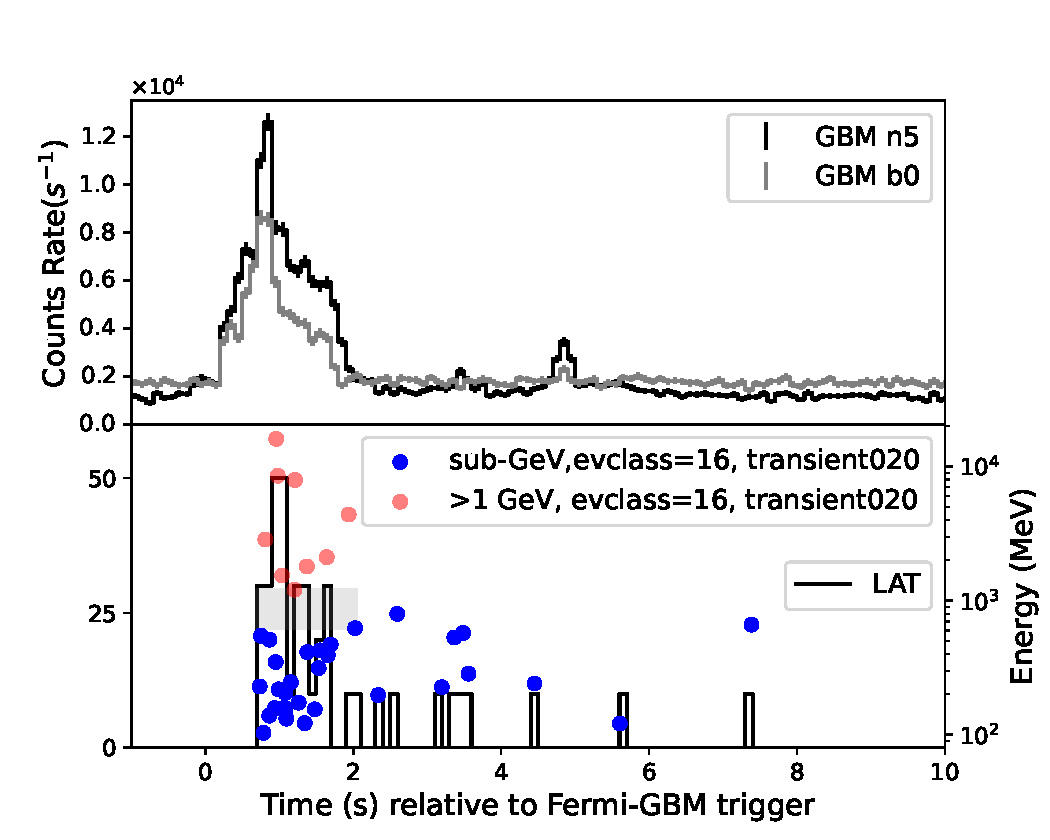
\includegraphics[width=.49\textwidth]{multi4.pdf}%\put(-100,125){(a) } \\
%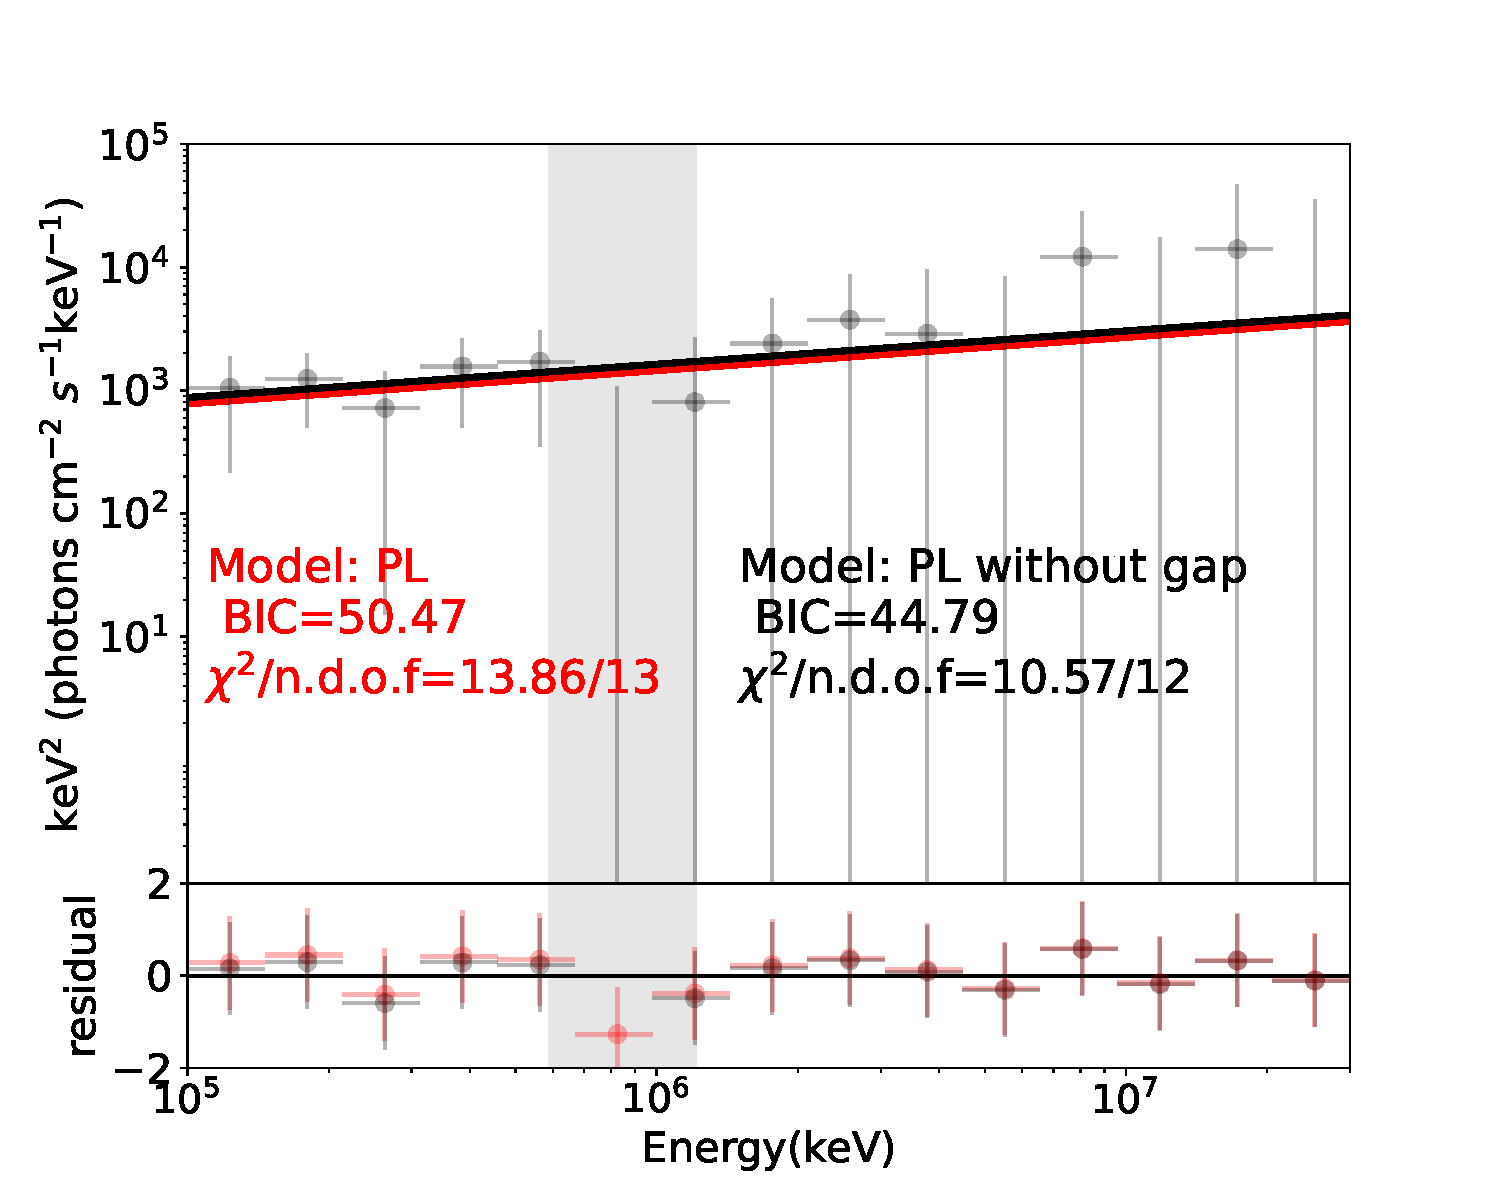
\includegraphics[width=.49\textwidth]{Fv_PL0_GRBHEB210704.pdf}\put(-100,125){(b)}
%{Fv_mBBBAND0_GRB210704A_withgapbin.pdf}\put(-100,130){(b)}
 \caption{\label{fig:spectra} (Color online) %(a) 
    Left Y-axis with the unit of counts rate (s$^{-1}$): the histograms are the light curves of GBM detectors (NaI 5 and BGO 0, upper plot) and LAT (bottom plot); the high-energy photons are from the LAT data of TRANSIENT020 class (or evclass=16), and used in the analysis to maximize the statistics for spectral analysis of GRB prompt emission. Right Y-axis with the unit of MeV in bottom plot: energies of high-energy photons (denoted by circles).  The gray shadow in the first 2 s denotes intersection of all gaps between sub-GeV (blue circles) and GeV (red circles) photons. 
    %(b) The time-integrated spectral modeling with PL function for high-energy photons, with and without considering zero-count in the gap (marked in gray).
    %(b) The time-integrated spectral modeling with mBB + BAND function, with considering 0-count in the gap (marked in gray).
    }
    \end{center}
\end{figure}

A full likelihood analysis is performed with \textsc{gtlike} \DIFdelbegin \DIFdel{, }\DIFdelend to quantify the statistical significance of this gap. Similarly to \cite{2016MNRAS.463.1144W}, we compared a continuous power-law (PL) model with a model explicitly incorporating a spectral gap~\footnote{For \textsc{gtlike}, a \DIFdelbegin \DIFdel{“}\DIFdelend \DIFaddbegin \DIFadd{``}\DIFaddend FileFunction\DIFdelbegin \DIFdel{” }\DIFdelend \DIFaddbegin \DIFadd{'' }\DIFaddend option is allowed for \DIFaddbegin \DIFadd{a }\DIFaddend fixed spectral shape and the sole parameter is a multiplicative normalization. To obtain the best parameter for \DIFaddbegin \DIFadd{the }\DIFaddend PL with a gap of \DIFdelbegin \DIFdel{0.6 to 1.2 }\DIFdelend \DIFaddbegin \DIFadd{$[0.64, 1.17]$ }\DIFaddend GeV, a parameter \DIFdelbegin \DIFdel{scanning }\DIFdelend \DIFaddbegin \DIFadd{scan }\DIFaddend is performed for \DIFdelbegin \DIFdel{each parameter (}\DIFdelend \DIFaddbegin \DIFadd{the }\DIFaddend index of \DIFdelbegin \DIFdel{power-law) and extract }\DIFdelend \DIFaddbegin \DIFadd{the power law; }\DIFaddend the minimum \DIFdelbegin \DIFdel{–log(likelihood) }\DIFdelend \DIFaddbegin \DIFadd{$-\log(\rm likelihood)$ }\DIFaddend and the error (the difference between \DIFaddbegin \DIFadd{the }\DIFaddend index \DIFdelbegin \DIFdel{of }\DIFdelend \DIFaddbegin \DIFadd{at }\DIFaddend the minimum \DIFdelbegin \DIFdel{–log(likelihood) }\DIFdelend \DIFaddbegin \DIFadd{$-\log(\rm likelihood)$ }\DIFaddend and that \DIFaddbegin \DIFadd{at $-\log({\rm likelihood})\pm0.5$) are extracted. The fits give $-\log({\rm likelihood})=39.18$ with an index }\DIFaddend of \DIFdelbegin \DIFdel{–log(}\DIFdelend \DIFaddbegin \DIFadd{$1.73\pm0.13$ for the continuous PL, and $-\log({\rm likelihood})=34.53$ with an index of $1.70^{+0.13}_{-0.12}$ for the PL with the gap. For this unbinned }\DIFaddend likelihood \DIFdelbegin \DIFdel{)+/-0.5)}\DIFdelend \DIFaddbegin \DIFadd{comparison, the changes in the Akaike and Bayesian information criteria are identical.}\DIFaddend }, and the analysis yields a preference for the gap model with \DIFdelbegin \DIFdel{$\Delta \mathrm{BIC=-2\Delta\rm{log(likelihood)}}=9.2$}\DIFdelend \DIFaddbegin \DIFadd{$\Delta \mathrm{BIC}=-2\Delta\log({\rm likelihood})=9.2$}\DIFaddend . This value constitutes strong statistical evidence against a simple continuous spectrum~\footnote{$\Delta \mathrm{BIC}$ between 2 and 6 indicates positive evidence; 6--10 indicates strong evidence; and $>10$ implies very strong evidence.}, further supporting the physical separation of the two emission components.\DIFaddbegin \DIFadd{~}\footnote{\DIFadd{A modeling with the PL plus a specific absorption-line profile (e.g., a Gaussian absorption line) was also attempted; however, the statistics of the events around the gap are not high enough to constrain the line parameters (the width, depth and central energy) well, which leads to overfitting by redundant parameters. Moreover, the central energy of the gap varies with time even within this short interval, so that a time-resolved analysis would be necessary to determine the parameters of a specific absorption line even with sufficient statistics.}} \DIFaddend Furthermore, a time-resolved analysis reveals that the upper energy envelope of the sub-GeV photons and the lower energy envelope of GeV photons evolve synchronously, maintaining the gap structure. This strong correlation ($\rho > 0.7$, Spearman rank; see the details in Appendix~\ref{sec: correlation}) suggests that the two components are physically linked but separated by an absorption mechanism.

%We quantified the significance of this gap using a Monte Carlo (MC) simulation. Assuming a continuous power-law (PL) distribution that connects the sub-GeV and GeV components, we generated $1.4 \times 10^5$ synthetic photon samples folded with the detector response. The probability of observing a gap width $\ge 590$ MeV (the intersection of all gaps in GeV emission in the first 2 seconds) in the time-intergrated spectrum purely due to Poisson fluctuations was determined to be $p$-value $< 10^{-3}$; this $p$-value is overestimated due to the smoothing effect of the time-intergrated spectrum on the gap. Considering the range of the gap that changes over time, the product of a sequence of $p$-values ($\prod p-$value) for the corresponding larger gaps in time-resolved spectra is very tiny ($\ll10^{-6}$, see details in Appendix~\ref{sec: probstudy}). Furthermore, a time-resolved analysis reveals that the upper energy envelope of the sub-GeV photons and the lower energy envelope of GeV photons evolve synchronously, maintaining the gap structure. This strong correlation ($\rho > 0.7$, Spearman rank; see the details in Appendix~\ref{sec: correlation}) suggests that the two components are physically linked but separated by an absorption mechanism. 


%To rigorously validate this spectral structure, we performed parameter estimation using Markov Chain Monte Carlo (MCMC) sampling with the \textsc{emcee} package~\cite{2013PASP..125..306F}. Similarly to \cite{2016MNRAS.463.1144W}, we compared a continuous power-law model with a model explicitly incorporating a spectral gap using the Bayesian Information Criterion (BIC). As illustrated in FIG.~\ref{fig:spectra} (b), the analysis yields a preference for the gap model with $\Delta \mathrm{BIC} \approx 5.7$.
%This value constitutes strong statistical evidence against a simple continuous spectrum~\footnote{$\Delta \mathrm{BIC}$ between 2 and 6 indicates positive evidence; 6--10 indicates strong evidence; and $>10$ implies very strong evidence.}, further supporting the physical separation of the two emission components.



\textit{Comoving Frame Energetics.}---To interpret the physical origin of the gap, we must determine the Lorentz factor $\Gamma$. A combined model of \DIFdelbegin \DIFdel{multicolor blackbody (mBB, e.g. see \mbox{%DIFAUXCMD
\cite[][]{2008ApJ...682..463P,2010ApJ...709L.172R,2018ApJ...866...13H}}\hskip0pt%DIFAUXCMD
) }\DIFdelend \DIFaddbegin \DIFadd{a multicolor blackbody \mbox{%DIFAUXCMD
\citep[mBB, e.g. see][]{2008ApJ...682..463P,2010ApJ...709L.172R,2018ApJ...866...13H} }\hskip0pt%DIFAUXCMD
}\DIFaddend plus a PL function \DIFdelbegin \DIFdel{~\mbox{%DIFAUXCMD
\citep{1993ApJ...413..281B}  }\hskip0pt%DIFAUXCMD
}\DIFdelend for the broad energy band is used to describe the spectrum of \DIFaddbegin \DIFadd{the }\DIFaddend prompt emission from \DIFaddbegin \DIFadd{the }\DIFaddend keV to GeV energy band; with \DIFdelbegin \DIFdel{a }\DIFdelend \DIFaddbegin \DIFadd{the }\DIFaddend lowest BIC and \DIFdelbegin \DIFdel{difference }\DIFdelend \DIFaddbegin \DIFadd{a difference of }\DIFaddend $\Delta \rm{BIC}=8.1$, it is statistically preferred over the other models (see details in Figure~\ref{fig:spectra2} in Appendix\DIFaddbegin \DIFadd{~}\DIFaddend \ref{sec:spectra2}).

%Using the method described in \cite{2012MNRAS.420..468P, 2024ApJ...961..137S} (see the detais in Appendix~\ref{sec: estiGamma}), we derived $\Gamma$ from the quasi-thermal component of the spectrum. %The estimated Lorentz factor evolves with time, peaking at $\Gamma \approx 300$ around the peak of luminosity and decaying to $\Gamma \approx 190$ one second later. 
With $z=2.34$, the \DIFdelbegin \DIFdel{Lorentz Factor is estimated to be $\gtrsim500$ around the peak flux with the photon of highest energy (16.09 GeV); the }\DIFdelend model-dependent method using the quasi-thermal component in the prompt phase proposes a \DIFaddbegin \DIFadd{coasting Lorentz factor in the }\DIFaddend range of 500 to 900 \DIFaddbegin \DIFadd{for the photospheric outflow }\DIFaddend (see the details in Appendix~\ref{sec: estiGamma}). \DIFdelbegin %DIFDELCMD < 

%DIFDELCMD <  %%%
%DIF < We can not rule out the explanation of the multi-component emission mechanism, in which the cutoff around 1 GeV is caused by pair production while GeV photons are contributed from early afterglow. The optical depth for pair production $\tau_{\gamma\gamma}>1$ of a $\sim1$ GeV photon requires $\Gamma<2000$ with the emission radius of $10^{12}$ cm (a larger radius requires a smaller upper limit of $\Gamma$); %however, even if the photon of highest energy (16.09 GeV) is from the early afterglow with a radius as large as $10^{15}$ cm, the lower limit of $\Gamma=260$ is required. Moreover, the peak of flux in the MeV band arrives almost simultaneously with that of high-energy photons, implying that the prompt high-energy emission has an internal origin~\citep{2011ApJ...730....1L,2011ApJ...733...22H}. The external shock model can hardly account for the almost simultaneous emission of GeV and sub-GeV photons~\citep{2011MNRAS.412..522B} and the correlation between them.
%DIF < We first rule out standard electromagnetic mechanisms. 
%DIF < A two-component jet model (a fast spine and slow sheath, see, e.g., Ref.~\cite{2025ApJ...995L...2A}) fails to explain the synchronized temporal evolution of the sub-GeV and GeV components. Similarly, Klein-Nishina suppression in Inverse Compton scattering would produce a high-energy cutoff rather than a discrete gap followed by a recovery in flux at $>1.2$ GeV.
%DIF < Therefore, we turn to photon-matter interactions.
\DIFdelend \DIFaddbegin \DIFadd{For the region emitting the GeV photons---in our picture a more external internal shock than that producing the MeV emission---the escape of the photon with the highest energy (16.09 GeV) through the MeV photon shell requires $\Gamma_{\rm G}\gtrsim4\times10^{2}$ at $R_{\rm G}\simeq3\times10^{12}$ cm (see the two-zone analysis in Appendix~\ref{sec:twozone}).
}\DIFaddend 


Applying the Doppler correction $E' \approx E_{\rm obs} (1+z) / 2\Gamma$ with $\Gamma=300$, the observed gap ([0.62, 1.21] GeV) translates to a comoving energy range of:
\begin{equation}
E_{\rm gap}^{\prime} \approx 3.5 - 6.7 \text{ MeV}.
\end{equation}
%DIF <  Even with $\Gamma=900$, the range is $1.2-2.2$ MeV. This energy range is critical.
\DIFaddbegin \DIFadd{For $\Gamma=430$, the value required by the escape of the 16.09 GeV photon in the two-zone configuration (Appendix~\ref{sec:twozone}), the range is $2.4-4.7$ MeV, still bracketing the deuterium resonance. Even with $\Gamma=900$, the range is $1.2-2.2$ MeV. This energy range is critical.
}

\DIFadd{Before attributing the gap to absorption by matter, we examine whether it could arise from intrinsic spectral evolution or from the superposition of different emission components, e.g. a cutoff of the prompt keV--GeV component at sub-GeV energies due to internal photon-photon absorption, with an early-afterglow component emerging at higher energies.
First, the pair-production optical depth increases monotonically with the photon energy above the threshold, so internal two-photon absorption would produce a high-energy cutoff rather than a discrete gap followed by a recovery in flux above 1.21 GeV. Quantitatively, for the Lorentz factors allowed by the escape of the highest-energy photon in the two-zone configuration (Appendix~\ref{sec:twozone}), the pair-production optical depth at the gap energies is far below unity; thus the deficit of photons in $[0.62, 1.21]$ GeV cannot be an absorption trough of pair production.
Second, the GeV photons are unlikely to originate from external shocks: in the external forward shock model, it takes a few seconds for the accelerated electrons to produce 100 MeV photons and a somewhat longer time to produce GeV photons~\mbox{%DIFAUXCMD
\citep{2011MNRAS.412..522B}}\hskip0pt%DIFAUXCMD
, so that the $\sim$GeV emission should be delayed with respect to the 100 MeV emission by about half of the deceleration time; however, the observed 100 MeV and GeV emissions arrive almost simultaneously. Case studies of GRB 090902B and GRB 090510 also suggest that the external shock model cannot interpret the prompt GeV data~\mbox{%DIFAUXCMD
\citep{2011ApJ...730....1L,2011ApJ...733...22H}}\hskip0pt%DIFAUXCMD
, and the modeling of \mbox{%DIFAUXCMD
\cite{2011MNRAS.415...77M} }\hskip0pt%DIFAUXCMD
indicates that the external shock model may interpret the GeV emission after, but not during, the prompt phase. For GRB 210704A, the high-energy prompt emission traces the MeV emission well (FIG.~\ref{fig:spectra}), implying an internal origin; moreover, the correlation between the GeV photons and the upper energy envelope of the sub-GeV photons would be difficult to explain if the GeV photons were from external shocks.
In addition, a two-component jet model (a fast spine and a slow sheath; see, e.g., \mbox{%DIFAUXCMD
\citealt{2025ApJ...995L...2A}}\hskip0pt%DIFAUXCMD
) fails to explain the synchronized temporal evolution of the sub-GeV and GeV components, and Klein-Nishina suppression in inverse Compton scattering would produce a high-energy cutoff rather than a discrete gap followed by a recovery in flux at $>1.21$ GeV.
Therefore, we turn to photon-matter interactions.
}\DIFaddend 


\textit{Resonant Nuclide Absorption.}---We propose that the gap arises from the resonant absorption of photons by nuclei entrained in the jet. The comoving energy of $\sim 4$ MeV aligns remarkably well with the photodissociation threshold of deuterium:
\begin{equation}
\gamma + {^2\text{H}} \rightarrow p + n.
\end{equation}
The cross-section for photodissociation peaks typically around $4-5$ MeV \cite{IAEA2000}, which perfectly matches our derived comoving energy $E_{\rm gap}^{\prime}$.

Crucially, this energy scale distinguishes deuterium from all other potential nuclear absorbers. Heavier nuclides, particularly the Fe-group elements often invoked in supernova models, interact with photons primarily through the Giant Dipole Resonance (GDR). The GDR peak energy for nuclei with mass number $A$ is approximately $E_{\rm GDR} \approx 31.2 A^{-1/3} + 20.6 A^{-1/6}$ MeV \cite{1975RvMP...47..713B}, which places the resonance at $15-25$ MeV for heavy elements (e.g., $^{56}$Fe) \cite{2020NuDS..163..109K}. Such absorption would manifest at observed energies $>3$ GeV, far above the gap detected in GRB 210704A. The unique low-energy threshold of deuterium makes it the only viable candidate for an absorption feature at $\sim 4$ MeV.

If the \DIFaddbegin \DIFadd{gap indeed arises from }\DIFaddend resonant deuterium absorption\DIFdelbegin \DIFdel{almost fix }\DIFdelend \DIFaddbegin \DIFadd{, the resonance energy in turn almost fixes }\DIFaddend the Lorentz factor \DIFdelbegin \DIFdel{being around 300, we }\DIFdelend \DIFaddbegin \DIFadd{of the emitting region to be around $(3-4)\times10^{2}$; we therefore }\DIFaddend choose $\Gamma = 10^{2.5}$ as a typical value in the following.
%DIF > %% TODO(team): the 16.09 GeV photon favors the upper end of this window (Gamma_G ~= 434, R_G ~= 3.4e12 cm, Appendix "two-zone"); there tau_gD from the formula below needs the per-pulse enhancement of L_K (or a larger Y_D) to remain >~ 1 -- reconcile with the adopted typical value Gamma = 10^2.5, or attribute the single 16 GeV photon to the upper end.

\textit{Timescales and Nucleosynthesis.} ---
With the standard internal shock model for the prompt emission, the emitting radius is determined to be~\citep{2011ApJ...726...90Z}
\DIFdelbegin \begin{displaymath}
%DIF < R_{\rm IS}=d/(\beta_{\rm f}-\beta_{\rm s})\simeq 2 \Gamma_{\rm s}^2 c \delta t \simeq 6 \times 10^{11} \Gamma_{\rm s,2}^2 \delta t_{-3} \ {\rm cm},
\DIFdel{R \simeq 2 \Gamma^2 c \delta t \simeq 6 \times 10^{12} \Gamma_{2.5}^2 \delta t_{-3}/(1+z) \ {\rm cm},
}\end{displaymath}%DIFAUXCMD
\DIFdelend \DIFaddbegin \begin{equation}\DIFadd{\label{eq:Ris}
%DIF > R_{\rm IS}=d/(\beta_{\rm f}-\beta_{\rm s})\simeq 2 \Gamma_{\rm s}^2 c \delta t \simeq 6 \times 10^{11} \Gamma_{\rm s,2}^2 \delta t_{-3} \ {\rm cm},
R \simeq 2 \Gamma^2 c \delta t/(1+z) \simeq 6 \times 10^{12} \Gamma_{2.5}^2 \delta t_{-3}/(1+z) \ {\rm cm},
}\end{equation}\DIFaddend 
%where $d=c\delta t$, $\delta t$ is the duration between the end of ejecting a leading slow shell and the beginning of ejecting a trailing fast shell, $\beta=v/c$, 's’ denotes the slow shell, while 'f’ denotes the fast shell.
\DIFdelbegin \DIFdel{To extract the time scale (}\DIFdelend \DIFaddbegin \DIFadd{where $\delta t$ is the timescale of the pulse duration; hereafter, the convention $Q_s = Q/10^s$ is adopted in cgs units throughout the text. To extract }\DIFaddend $\delta t$\DIFdelbegin \DIFdel{) of pulse duration}\DIFdelend , a wavelet decomposition is performed with the data of the internal shock emission (photons of energy $< 20$ keV are required, and the contribution from \DIFaddbegin \DIFadd{the }\DIFaddend quasi-thermal emission is $7\%$\DIFdelbegin \DIFdel{. The }\DIFdelend \DIFaddbegin \DIFadd{; the }\DIFaddend light curve has a sampling rate of 4000 Hz; see the details of the method in \DIFdelbegin \DIFdel{~\mbox{%DIFAUXCMD
\citep[][]{2013MNRAS.432..857M}}\hskip0pt%DIFAUXCMD
}\DIFdelend \DIFaddbegin \DIFadd{\mbox{%DIFAUXCMD
\citealt{2013MNRAS.432..857M}}\hskip0pt%DIFAUXCMD
}\DIFaddend ). $\delta t$ is determined to be about 1 ms with an uncertainty of a few ms. Considering the redshift ($z=2.34$), the emitting radius \DIFaddbegin \DIFadd{is }\DIFaddend $R \sim 2 \times 10^{12}$ cm.
%For the slow shell with a small $\Gamma_{\rm s}\sim100$, $R_{\rm IS}\sim 10^{11}$ cm is possible.

The identification of deuterium is further supported by the dynamical timescales of the GRB jet. %The prompt emission occurs at a radius $R \sim 10^{13}-10^{14}$ cm. %ref
The dynamical time in the comoving frame is extremely short, \DIFdelbegin \DIFdel{on the order of hundreds of seconds}\DIFdelend \DIFaddbegin \DIFadd{only a fraction of a second}\DIFaddend :
\begin{equation}
t'_{\rm dyn} \approx \frac{R}{\Gamma c} \sim 0.1 R_{12} \Gamma_{2.5}^{-1} \text{ s}.
\end{equation}
In a neutron-rich outflow ejected from \DIFdelbegin \DIFdel{a merger}\DIFdelend \DIFaddbegin \DIFadd{the central engine}\DIFaddend , nucleosynthesis begins with the rapid capture of neutrons by protons ($p + n \rightarrow {^2\text{H}}$). To form heavier $r$-process elements (up to \DIFdelbegin \DIFdel{Lanthanides}\DIFdelend \DIFaddbegin \DIFadd{lanthanides}\DIFaddend ), the chain must proceed through the creation of seed nuclei. However, the formation of seeds heavier than deuterium is rate-limited by weak interactions ($\beta$-decays), which typically require timescales of seconds to minutes to proceed significantly\DIFdelbegin \DIFdel{. 0.1 s is }\DIFdelend \DIFaddbegin \DIFadd{; a timescale of $\sim0.1$ s is far }\DIFaddend too short for heavier elements to form. %On the other hand, for the kilonova side, the $r$-process in the non-relativistic outflow is not influenced by such a jet effect, and lanthanides and other heavy elements still form \cite{2017Natur.551...80K}.

Given the relativistic expansion, the jet material is ``frozen out" before significant quantities of heavy elements can form via $\beta$-decay. Consequently, the jet composition at the photospheric radius is expected to be dominated by nucleons and light isotopes, specifically deuterium, rather than heavy metals. This kinetic constraint robustly %excludes Fe-group elements and 
reinforces the deuterium interpretation.

\textit{Optical depths for photon-electron and photon-deuteron interactions in relativistic internal shocks.}--- The comoving density of the jet, mainly contributed by protons (with a rest mass of $m_p$), is expressed in terms of the isotropic matter luminosity (\DIFdelbegin \DIFdel{$L_{\rm K}=E_{\rm K}/T_{\rm dur,\\lab}$}\DIFdelend \DIFaddbegin \DIFadd{$L_{\rm K}=E_{\rm K}/T_{\rm dur,lab}$}\DIFaddend ; $E_{\rm K}$ is the kinetic energy \DIFdelbegin \DIFdel{, $T_{\rm dur,\\lab}$ }\DIFdelend \DIFaddbegin \DIFadd{and $T_{\rm dur,lab}$ }\DIFaddend is the duration time in the lab frame) of the jet at the non-thermal emission radius $R$ as%~\footnote{in the comoving frame, the shell volume is $V'=4\pi R^2 (R/\Gamma)$; one has $n^{\prime}_{p}V'm_pc^2=M_{\rm iso}c^2$ and $E_{\rm K}=\Gamma M_{\rm iso} c^2$}
\DIFdelbegin \begin{align*}\DIFdel{%DIFDELCMD < \label{eq:nbp}%%%
 n^{\prime}_{p}=\frac{L_{\rm K}}{4\pi R^2 c \Gamma^2 m_p c^2}\nonumber
     =1.8\times 10^{17} L_{\rm K,55} R_{12}^{-2}\Gamma_{2.5}^{-2} \ \rm cm^{-3} , \nonumber}\\
\DIFdel{}\end{align*}%DIFAUXCMD
\DIFdelend \DIFaddbegin \begin{equation}\DIFadd{\label{eq:nbp}
 n^{\prime}_{p}=\frac{L_{\rm K}}{4\pi R^2 c \Gamma^2 m_p c^2}
     =1.8\times 10^{17} L_{\rm K,55} R_{12}^{-2}\Gamma_{2.5}^{-2} \ {\rm cm^{-3}},
}\end{equation}\DIFaddend 
where $L_{\rm K,55}=L_{\rm K}/10^{55}{\,\rm erg\,s^{-1}}$ and the unit of $R$ is cm\DIFdelbegin \DIFdel{; in the following, the convention $Q_s = Q/10^s$ is adopted in cgs units throughout the text}\DIFdelend . With the comoving density of deuterium $n'_{D}$ and the number fraction of deuterium ($Y_{D}$),
the optical depth for the photodissociation of deuterium is 
\begin{equation}\label{eq:taugD}
  \tau_{\gamma D}\sim\frac{\sigma_{\gamma D} n'_ D R}{\Gamma}=1.4 Y_{D} L_{\rm K, 55} R_{12}^{-1} \Gamma_{2.5}^{-3},
\end{equation}
where $\sigma_{\gamma D}\simeq 2.5\times10^{-27}$ cm$^{2}$ at a photon energy
$\varepsilon'_\gamma \simeq 4.48~{\rm MeV}$ in the deuteron rest frame \cite{IAEA2000}. %Page 71, 1st line. Citation there: Ann.Phys.27,79,1964, Fuller
%Note that  $\Gamma\simeq 500$ is taken for the merged shells in internal shocks; it is typically less than the estimated maximum value.  

On the other hand, the GeV photons should \DIFdelbegin \DIFdel{be freely escaped }\DIFdelend \DIFaddbegin \DIFadd{escape freely }\DIFaddend from the scattering \DIFdelbegin \DIFdel{of }\DIFdelend \DIFaddbegin \DIFadd{off }\DIFaddend electrons. Internal shocks are natural sites for the dissipation of the kinetic energy of a baryonic fireball~\citep[][]{1990ApJ...365L..55S,1992MNRAS.258P..41R,1993ApJ...405..278M,1994ApJ...430L..93R}.
In the internal shock model of gamma-ray bursts, electrons accelerated at relativistic shocks are commonly assumed to follow a non-thermal distribution \cite{2004RvMP...76.1143P}\DIFdelbegin \DIFdel{.
}\DIFdelend \DIFaddbegin \DIFadd{,
}\DIFaddend \begin{equation}
N(\gamma_e) \propto \gamma_e^{-p}, \qquad \gamma_e \ge \gamma_m ,
\end{equation}
where $\gamma_m$ is the minimal Lorentz factor of the electrons accelerated in the internal shocks.
For typical internal shock parameters adopted in the literature, $\gamma_m \sim 10^{3.5}$--$10^6$ \cite{2013ApJ...769...69B,2019A&A...628A..59O}. The scattering regime between photons and relativistic electrons is determined by
\begin{equation}
x \equiv \frac{\gamma_e \varepsilon'_\gamma}{m_e c^2},
\end{equation}
where $\varepsilon'_\gamma$ is the photon energy in the comoving frame. One has $x \gtrsim 8\times 10^5$ for $\varepsilon_\gamma'\sim4$ MeV and $\gamma_m\simeq 10^{5}$ as typical values. In this Klein-Nishina limit, the total scattering cross section is suppressed to \cite{1986rpa..book.....R}
\begin{equation}
\sigma_{\rm KN} \simeq 
\frac{3}{8}\sigma_T
\frac{\ln(2x)+1/2}{x} 
\lesssim 4.6 \times 10^{-30}\ \ {\rm cm}^2,
\label{eq:sigmaKN-GBM}
\end{equation}
thus, the optical depth for Compton scattering in the Klein-Nishina regime is
\DIFdelbegin \DIFdel{about 
}\begin{displaymath}
\DIFdel{\tau_{\rm KN} \sim \frac{\sigma_{\rm KN} n'_e R}{\Gamma}
\lesssim 2.6\times10^{-3} L_{\rm K, 55}R_{12}^{-1} \Gamma_{2.5}^{-3}\ll 1,
%DIFDELCMD < \label{eq:sigmaKN-GBM}%%%
}\end{displaymath}%DIFAUXCMD
\DIFdelend \DIFaddbegin \begin{equation}
\DIFadd{\tau_{\rm KN} \sim \frac{\sigma_{\rm KN} n'_e R}{\Gamma}
\lesssim 2.6\times10^{-3} L_{\rm K, 55}R_{12}^{-1} \Gamma_{2.5}^{-3}\ll 1,
\label{eq:tauKN-GBM}
}\end{equation}\DIFaddend 
\DIFdelbegin \DIFdel{with assuming local electrical }\DIFdelend \DIFaddbegin \DIFadd{assuming local electric }\DIFaddend neutrality in the jet, $n'_{e}\simeq n'_p$.
%The break energy ($\varepsilon_b$) in the spectrum of the non-thermal component described by a BAND function (e.g. the synchrotron emission by the relativistic electrons in magnetic field) may correspond to $\tau_{\rm KN} (\varepsilon_b')\sim1$ at $\gamma_e\sim\gamma_m$. From the results of the modeling of the non-thermal component, the break energy is $\varepsilon_b\sim10^4$ keV, which corresponds to $\gamma_m\sim10^{5.4}$ in this case; $\sigma_{\rm KN}\sim10^{-30}$ cm$^{2}$ is much lower for the photons of $\varepsilon_\gamma'=4$ MeV, due to a deeper Klein-Nishina regime.

The \DIFdelbegin \DIFdel{estimations }\DIFdelend \DIFaddbegin \DIFadd{estimates }\DIFaddend above show that the \DIFdelbegin \DIFdel{GeV photons at the gap }\DIFdelend \DIFaddbegin \DIFadd{photons falling in the resonant band }\DIFaddend should be absorbed by the deuterium\DIFaddbegin \DIFadd{, }\DIFaddend while the other photons are able to escape from the scattering \DIFdelbegin \DIFdel{of }\DIFdelend \DIFaddbegin \DIFadd{off }\DIFaddend the electrons.%However, the MeV photons may not be able to escape as it may not be in the deep KN region.
%...
%Please note that "the MeV photons may not be able to escape" is not consistent with the observation. The PL component extends to keV region.


\textit{Discussion.}---Let us demonstrate
the plausibility of the observation of photodissociation of deuterium in the jet of GRB 210704A as follows: the \DIFaddbegin \DIFadd{first }\DIFaddend key point is whether \DIFaddbegin \DIFadd{the }\DIFaddend baryon loading in a relativistic outflow could produce enough deuterium;
second, GeV photons are emitted while those in the resonant \DIFdelbegin \DIFdel{regions }\DIFdelend \DIFaddbegin \DIFadd{region }\DIFaddend are absorbed by deuterium, which requires that $\tau_{\gamma D}$ and $\tau_{\rm KN}$ (for GeV photons) \DIFdelbegin \DIFdel{should }\DIFdelend satisfy
\begin{equation}\label{eq:criterion}
    \tau_{\rm KN}<1\lesssim\tau_{\gamma D}.
\end{equation}

The total \DIFdelbegin \DIFdel{energy }\DIFdelend \DIFaddbegin \DIFadd{isotropic-equivalent luminosity }\DIFaddend of the outflow could be estimated \DIFdelbegin \DIFdel{by the radiative $E_{\gamma, \rm iso}$ }\DIFdelend \DIFaddbegin \DIFadd{from the radiated luminosity $L_{\gamma, \rm iso}$ }\DIFaddend and the radiative efficiency ($\epsilon_\gamma$) as
\DIFdelbegin \begin{displaymath}
    \DIFdel{E_{\rm tot, iso}= E_{\gamma, \rm iso}/\epsilon_\gamma;
}\end{displaymath}%DIFAUXCMD
\DIFdelend \DIFaddbegin \begin{equation}
    \DIFadd{L_{\rm tot, iso}= L_{\gamma, \rm iso}/\epsilon_\gamma;
}\end{equation}\DIFaddend 
for \DIFaddbegin \DIFadd{a }\DIFaddend baryonic fireball, $L_{\rm K}\lesssim (1-\epsilon_\gamma)L_{\rm tot, iso}$.
It is reasonable that $\epsilon_\gamma\lesssim10\%$, \DIFdelbegin \DIFdel{and this is }\DIFdelend because the radiation efficiency of internal shocks is typically low \DIFdelbegin \DIFdel{(e.g., see Refs.~\mbox{%DIFAUXCMD
\citep[][]{2011ApJ...726...90Z,2008FrPhC...3..306F}}\hskip0pt%DIFAUXCMD
)}\DIFdelend \DIFaddbegin \DIFadd{\mbox{%DIFAUXCMD
\citep[e.g.,][]{2011ApJ...726...90Z,2008FrPhC...3..306F}}\hskip0pt%DIFAUXCMD
}\DIFaddend . $L_{\gamma, \rm iso}=1.0\times10^{54}$ erg s$^{-1}$ for the component from \DIFaddbegin \DIFadd{the }\DIFaddend keV to GeV energy band (about 2.6 times that of the peaking component in \DIFaddbegin \DIFadd{the }\DIFaddend MeV emission); therefore, we assume that $L_{\rm K}$ is comparable to \DIFdelbegin \DIFdel{$ 10^{55}$ }\DIFdelend \DIFaddbegin \DIFadd{$10^{55}$ }\DIFaddend erg s$^{-1}$.
In fact, $L_{\gamma, \rm iso}$ obtained from the modeling is time-averaged; the density of baryons is not uniform, and $L_{\rm K}$ for each pulse (or shell) is even larger.


$Y_{D}$ can be as large as $\simeq10\%$ under the right conditions in neutron-ion decoupling \DIFdelbegin \DIFdel{(see the simulation of Ref.~\mbox{%DIFAUXCMD
\citep[][]{2002ApJ...580..368P}}\hskip0pt%DIFAUXCMD
). The }\DIFdelend \DIFaddbegin \DIFadd{\mbox{%DIFAUXCMD
\citep[see the simulation in][]{2002ApJ...580..368P}}\hskip0pt%DIFAUXCMD
. A }\DIFaddend large production of deuterium could \DIFdelbegin \DIFdel{be }\DIFdelend \DIFaddbegin \DIFadd{also proceed }\DIFaddend through the spallation
of $\alpha$-particles~\citep{2003ApJ...588..931B}, which is caused by neutron-ion decoupling, as well as \DIFaddbegin \DIFadd{by }\DIFaddend internal shocks.
\DIFdelbegin \DIFdel{In }\DIFdelend \DIFaddbegin \DIFadd{Although nucleosynthesis is sensitive to the unknown details of }\DIFaddend the intense internal shocks \DIFdelbegin \DIFdel{that occur }\DIFdelend \DIFaddbegin \DIFadd{occurring }\DIFaddend in the jet of GRB 210704A, \DIFdelbegin \DIFdel{although nucleosynthesis is sensitive to
these unknown details inside, }\DIFdelend we expect that $Y_{D}$ might be even greater due to the spallation of $\alpha$-particles. Considering that the fraction of $\alpha$-particles could be comparable with \DIFdelbegin \DIFdel{those }\DIFdelend \DIFaddbegin \DIFadd{that }\DIFaddend of nucleons for the short \DIFdelbegin \DIFdel{dynamic }\DIFdelend \DIFaddbegin \DIFadd{dynamical }\DIFaddend time~\citep[]{2002ApJ...580..368P,2003ApJ...588..931B}, $Y_{\rm D}\simeq0.3$ is not impossible and Eq\DIFaddbegin \DIFadd{.~}\DIFaddend (\ref{eq:criterion}) is satisfied in this case. For the Lorentz \DIFdelbegin \DIFdel{Factor}\DIFdelend \DIFaddbegin \DIFadd{factor}\DIFaddend , $\Gamma\simeq 300$ is a plausible value that could lead to $\tau_{\gamma D}\gtrsim1$.
Given $\gamma_m\simeq5\times10^{6}$ and $p=2$ \DIFdelbegin \DIFdel{of }\DIFdelend \DIFaddbegin \DIFadd{for }\DIFaddend the power-law distribution of $\gamma_e$, \DIFdelbegin \DIFdel{for }\DIFdelend \DIFaddbegin \DIFadd{even }\DIFaddend photons of much smaller energy, e.g. $E_{\rm obs}\simeq10$ keV, \DIFdelbegin \DIFdel{this satisfies }\DIFdelend \DIFaddbegin \DIFadd{satisfy }\DIFaddend $\tau_{\rm KN}<1$. This is well consistent with the observed prompt spectrum.

%\iffalse
 For the high-energy photons, because of the very small optical depth for Compton scattering, \DIFdelbegin \DIFdel{photons of PL component are emitted out of }\DIFdelend \DIFaddbegin \DIFadd{the photons of the PL component escape from }\DIFaddend the outflow once produced. The interactions between \DIFaddbegin \DIFadd{the }\DIFaddend high-energy photons and their target photons with lower energies are in the relativistic regime; thus the Lorentz factor of the outgoing pairs \DIFaddbegin \DIFadd{is }\DIFaddend $\gamma_{\pm}\gg1$ (where $\gamma_{\pm}\equiv\frac{E_{0}}{m_e c^2}$ and $E_{0}$ is the incoming photon
energy in the center-of-momentum frame), \DIFaddbegin \DIFadd{and }\DIFaddend the cross section for pair production is suppressed to\DIFdelbegin \DIFdel{be ~\mbox{%DIFAUXCMD
\citep{1976tper.book.....J, 2018pgrb.book.....Z}
}\hskip0pt%DIFAUXCMD
,
}\begin{displaymath}
\DIFdel{\sigma_{\gamma\gamma}=\frac{3}{8}\sigma_{\rm T} \gamma_{\pm}^{-2}(\rm{ln}2\gamma_{\pm}^2 -1)\simeq10^{-31} \ }\\\DIFdel{\rm{cm}^{2}\ll \sigma_{\rm T}.
}\end{displaymath}%DIFAUXCMD
\DIFdelend \DIFaddbegin \DIFadd{~\mbox{%DIFAUXCMD
\citep{1976tper.book.....J, 2018pgrb.book.....Z}
}\hskip0pt%DIFAUXCMD
}\begin{equation}
\DIFadd{\sigma_{\gamma\gamma}=\frac{3}{8}\sigma_{\rm T} \gamma_{\pm}^{-2}(}{\DIFadd{\rm ln}}\DIFadd{2\gamma_{\pm}^2 -1)\simeq10^{-31} \ {\rm cm}^{2}\ll \sigma_{\rm T}.
}\end{equation}\DIFaddend 
$\tau_{\gamma\gamma}\lesssim1$ \DIFdelbegin \DIFdel{of }\DIFdelend \DIFaddbegin \DIFadd{for }\DIFaddend the high-energy photons of 1.21 GeV$-$4.39 GeV\DIFdelbegin \DIFdel{which consist of the upper envelope }\DIFdelend \DIFaddbegin \DIFadd{, which constitute the upper boundary }\DIFaddend of the gap, requires \DIFdelbegin \DIFdel{that }\DIFdelend $\Gamma\gtrsim300$ at $R\sim10^{12}$ cm, which is \DIFdelbegin \DIFdel{consistent well }\DIFdelend \DIFaddbegin \DIFadd{well consistent }\DIFaddend with our hypothesis.





%\fi

%The baryon loading mass in the jet is calculated to be $f_{b}M_{\rm iso}\sim10^{-6}M_{\odot}$ by $E_{\rm K}=\Gamma M_{\rm iso}c^2$ (the typical beaming factor for short GRBs is $f_b\sim6\times10^{-3}$, see~\citep[][]{2014ARA&A..52...43B}), which is a reasonable value for merger events~\citep{2007PhR...442..166N,2019LRR....23....1M,2025PhRvD.111f3040S}.

\textit{Conclusion.}---We identified a statistically significant spectral gap in the prompt emission of GRB 210704A. Interpreting this \DIFaddbegin \DIFadd{for the first time }\DIFaddend as resonant absorption by deuterium nuclei in a jet with $\Gamma\simeq 300$\DIFdelbegin \DIFdel{for the first time}\DIFdelend , we find a consistent physical picture that links the burst to a neutron-rich progenitor. This represents the first direct spectroscopic detection of \DIFdelbegin \DIFdel{nucleosynthesis ingredients in the }\DIFdelend \DIFaddbegin \DIFadd{the ingredients of }\DIFaddend $r$-process \DIFaddbegin \DIFadd{nucleosynthesis }\DIFaddend in the prompt gamma-ray phase, opening a new window for studying nuclear astrophysics in extreme environments.


Previous studies of GRB 210704A noted its peculiar properties, despite its duration lying in the intermediate range \citep{2021GCN.30380....1M, 2023MNRAS.522.5204B, 2026MNRAS.548ag555P}. %Our finding provides a completely independent confirmation of this progenitor channel. 
Unlike kilonovae, which probe the sub-relativistic ejecta days after the event, this spectral feature probes the relativistic jet itself seconds after launch, revealing the initial chemical composition of the $r$-process flow. It should be noted that such observations are expected to be rare\DIFdelbegin \DIFdel{. }\DIFdelend \DIFaddbegin \DIFadd{: }\DIFaddend GRB 210704A is a `short' long burst that favors the abundance of deuterium\DIFdelbegin \DIFdel{; }\DIFdelend \DIFaddbegin \DIFadd{, and }\DIFaddend the high baryon loading of the outflow \DIFdelbegin \DIFdel{and }\DIFdelend \DIFaddbegin \DIFadd{together with the }\DIFaddend rapid variability of the central engine \DIFdelbegin \DIFdel{create }\DIFdelend \DIFaddbegin \DIFadd{creates the }\DIFaddend conditions for the occurrence of intense internal shocks.




%Key findings are the following. 1. Discovery of a Spectral Gap: A statistically significant ``zone of avoidance" was detected between 0.62 GeV and 1.21 GeV photons during the prompt phase. 2. Comoving Energy Mapping: By constraining the bulk Lorentz factor to $\Gamma \approx 200–300$, the observed gap translates to a comoving energy of $\sim$4–7 MeV. 3. Identification of Deuterium: This energy range aligns perfectly with the photodissociation threshold of deuterium ($^2$H), which peaks around 4–5 MeV. 4. Progenitor Link: The presence of deuterium confirms that the jet was loaded with neutron-rich material, reinforcing a binary neutron star (BNS) or neutron star-black hole (NSBH) merger origin.

%The conclusion of this study is supported by a highly self-consistent physical framework that aligns across four key dimensions. First, there is a unique matching of energy scales: the observed $\sim$1 GeV spectral gap translates to a comoving energy of $\sim$4–7 MeV, which fits the photodissociation threshold of deuterium perfectly, whereas heavier elements (like the Fe-group) interact via the Giant Dipole Resonance at much higher comoving energies of 15–25 MeV. Second, the jet's extremely short comoving dynamical timescale of hundreds of seconds provides a natural bottleneck; while $p+n \rightarrow {}^2H$ can occur rapidly, the formation of heavier $r$-process elements is limited by slower $\beta$-decays, effectively ``freezing" the jet composition at the deuterium stage. Finally, the model follows a coherent opacity logic where, despite high baryon loading, the electron scattering is suppressed by the Klein-Nishina effect, creating a specific window where the jet is transparent to electrons ($\tau_{\gamma e} \approx 0.06$) but remains opaque to deuterium absorption ($\tau_{\gamma D} \sim 1$).
\section*{Acknowledgements}
%\begin{acknowledgments}
The authors are very grateful for the public GRB data from Fermi/GBM and Fermi/LAT. Dr. X.Y. Song thanks the support of the National Natural Science Foundation of China (grant No.12303052). Q. Liu and Dr. X.Y. Song are very grateful for the support from China's Space Origins Exploration Program. Prof. B.Q. Ma and Q. Liu appreciate the support of the National Natural Science Foundation of China (grant No.12335006). The authors thank anonymous reviewers for their useful comments. The authors thank Prof. Shuang-Nan Zhang, Prof. Ming-Yu Ge, and Prof. Francesco Longo for useful comments and discussions on the data analysis.
%\end{acknowledgments}

\iffalse
\textit{Note added.}—
While this work was under review, we became aware of a follow-up observation work on GRB 210704A was published \cite{2026MNRAS.548ag555P}. Some weak evidences the spectral energy distribution fit parameters, late-time imaging, as well as the GRB’s energetics, spectral lag, and location point to a collapsar nature. However, there were some contrary evidences point to a merger origin, such as extended emission (EE-GRBs) nature, non-detection of a confirmed supernova component. There was no decisive conclusion drawn whether it is from a collapsar or a merger.
Its optical afterglow is also unusual. As shown in Figure 10 of \cite{2026MNRAS.548ag555P}, there is a rebrightening at around around 1.8 days, which was classified into luminous fast blue optical transients (FBOT). The total energy of the FBOT is around $3.7 \times 10^{49}$ erg. The origin is also not clear. 
Interestingly, the light curve can be well explained in the resonant deuterium absorption scenario. 
As in the reaction, the deuterium splits into a proton and neutron, and the neutron will decays into a proton and an electron with half life time 7.5 minutes in the comoving frame. In special relativity, the time dilutes to around 1.56 days, with Lorentz factor being 300.
The total optical energy comes from the absorbed (0.62, 1.21) GeV photons, which is around $10^{51}$ erg (isotropic-equivalent). Considering some efficiency by transferring the GeV photon to the optical photons, the decayed secondary neutrons could power such an FBOT.
\fi

\appendix
%\section{APPENDIX}
\iffalse
\section{The probability study of the gap }\label{sec: probstudy}
The energy spectrum of high-energy photons detected in LAT could be described by a continuous PL function with index $p$, 
\begin{equation}\label{func:PL}
N_{\rm PL}(E)=A E^{-p}.
\end{equation}
%In the modeling, $p\simeq-1.7$ and the time-averaged flux of $1.8\times10^{-5}$ erg cm$^{-2}$ s$^{-1}$ are determined with high-energy data from $0.7$ to 2.0 s after the GBM trigger time ($T_0$).
\begin{figure}
\begin{center}
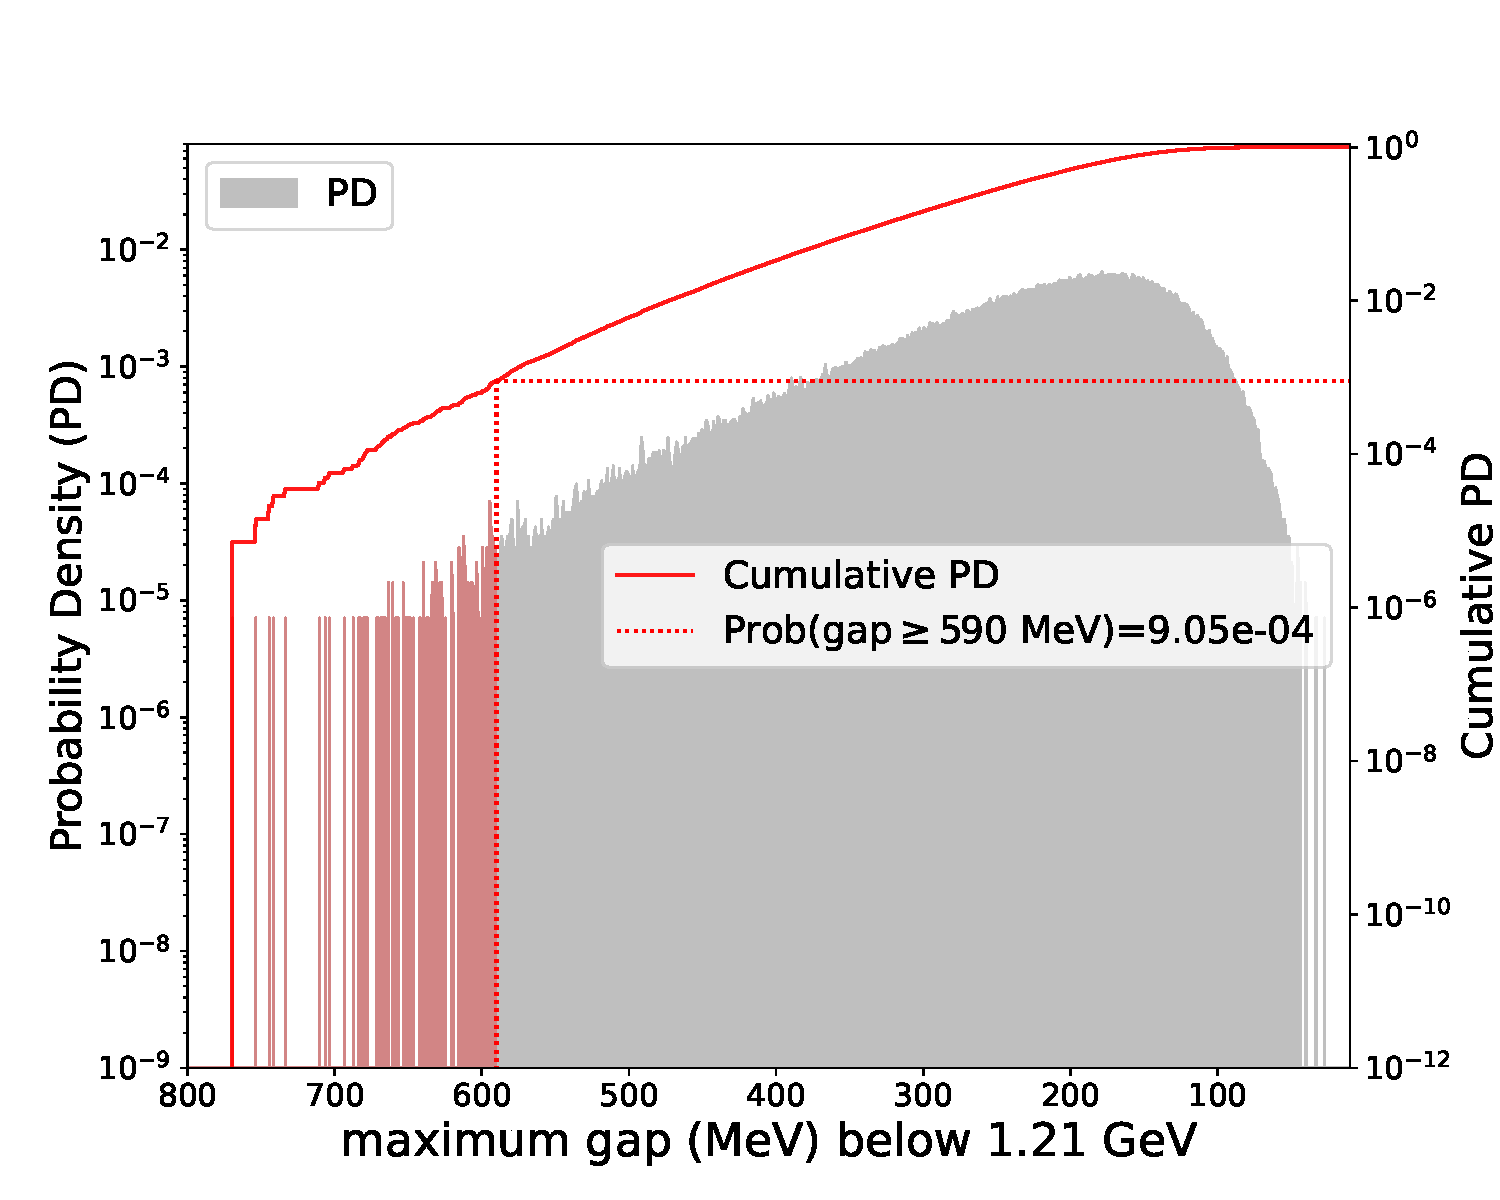
\includegraphics[width=.49\textwidth]{gapdis_hist_siglevel.pdf}\\
\caption{ PD (the gray shadow) of maximum gaps in photons below 1.21 GeV and cumulative PD (the solid red line). The $p$-value of the maximum gap $\geq 590$ MeV is labeled by the dotted red line, which is determined by the cumulative PD in red shadow.\label{fig:PD}}
 \end{center}
\end{figure}

\begin{table*} 
\centering
%\tiny  % 设置字体大小为 small
\caption{Time-resolved gaps and $p$-values.\label{tab:gapprob}}
\begin{ruledtabular}
\begin{tabular}{lccccc}
Time bins relative to trigger time (s)
&[0.70, 0.90]
&[0.90, 1.20]
&[1.20, 1.40]
&[1.40, 1.65]
&[1.65, 2.05]
%&$\prod_s \prod_i f(N^{\mathrm{mod}}_{i,s}, N^{\mathrm{obs}}_{i,s}=0)$
\\
Gap range (MeV) 
&[2860, 550]
&[1540, 350]
&[1210, 410]
&[2110, 430]
&[4390, 620]
\\
%\hline
 %index $p$ fixed to TI results & & &$1.74\pm{0.10}$&&\\
 $p$-value &0.0037 &0.0006 &0.0180 &0.0067 &0.0034 \\
%$N^{\mathrm{mod}}_{i,s}$, $f(N^{\mathrm{mod}}_{i,s},N^{\mathrm{obs}}_{i,s}= 0)$ of gap  &2.23,0.107&4.9,0.007&1.99,0.137&1.68,0.186&1.51,0.22&$4.5\times10^{-6}$\\
%$N^{\mathrm{mod}}$ and $f$  above GeV-line &0.72,0.489&2.38,0.262&1.61,0.322&0.64,0.525&0.3,0.741&$1.6\times10^{-2}$\\
\end{tabular}
\end{ruledtabular}
\end{table*}

A hypothesis testing for the continuous PL modeling of the high energy emission is performed, and the \textit{null hypothesis} is set to be that the statistical fluctuation could account for the gap of $[0.62,1.21]$ GeV; the test statistic is maximum gaps below an upper limit of $E_{\rm up}=1.21$ GeV.
A Monte-Carlo (MC) simulation is performed and $1.4\times10^5$ samples of the same total number of photons are generated based on the time-integrated spectrum of real data in $T_0+[0.70,2.05]$ s; note that the folded model with the response from the detector is used. The probability density (PD) distribution of the maximum gaps is extracted, as shown in FIG~\ref{fig:PD}. The probability of a gap width of $\geq590$ MeV for photons below 1.21 GeV is determined to be $<10^{-3}$, thus the \textit{ null hypothesis} that statistical fluctuation could explain the gap of $[0.62,1.21]$ GeV is rejected at a level of significance of $\alpha=0.001$, or the corresponding $p$-value is 0.001. 


In fact, the range of the gap varies over time and in the time-integrated spectrum it is the intersection of all, which is the smallest. Thus, we should consider the smoothing effect of the time-integrated spectrum on the gap; the $p$-value for the gap is overestimated in the case of time-integrated analysis.  %In time-resolved analysis, the expected number of photons in the folded model in the energy bins (with index $i$) of gaps for each slice (with index $s$) is denoted as $N^{\mathrm{mod}}_{i,s}$. The probability of the gaps due to the statistical fluctuation is derived as
Similar procedures are performed in time-resolved analysis, with the spectral index fixed to that of time-integrated modeling. As shown in TABLE.~\ref{tab:gapprob}, the lowest $p$-value is $6\times10^{-4}$ in $T_0+[0.9, 1.2]$ s, which is less than that of the time-integrated analysis; the product of a sequence of $p$-values ($\prod p-$value) is very tiny ($\ll10^{-6}$) considering the width of the gap that changes over time.


%$\rm Prob_{\rm gap}$ between GeV and sub-GeV is determined to be less than $5\times10^{-6}$, which is very small. %Note that the other gaps among the GeV photons have a much larger probability of $\sim10^{-2}$, which implies that they are not inconsistent with \textit{the null hypothesis}.
\fi

\begin{figure}
\begin{center}
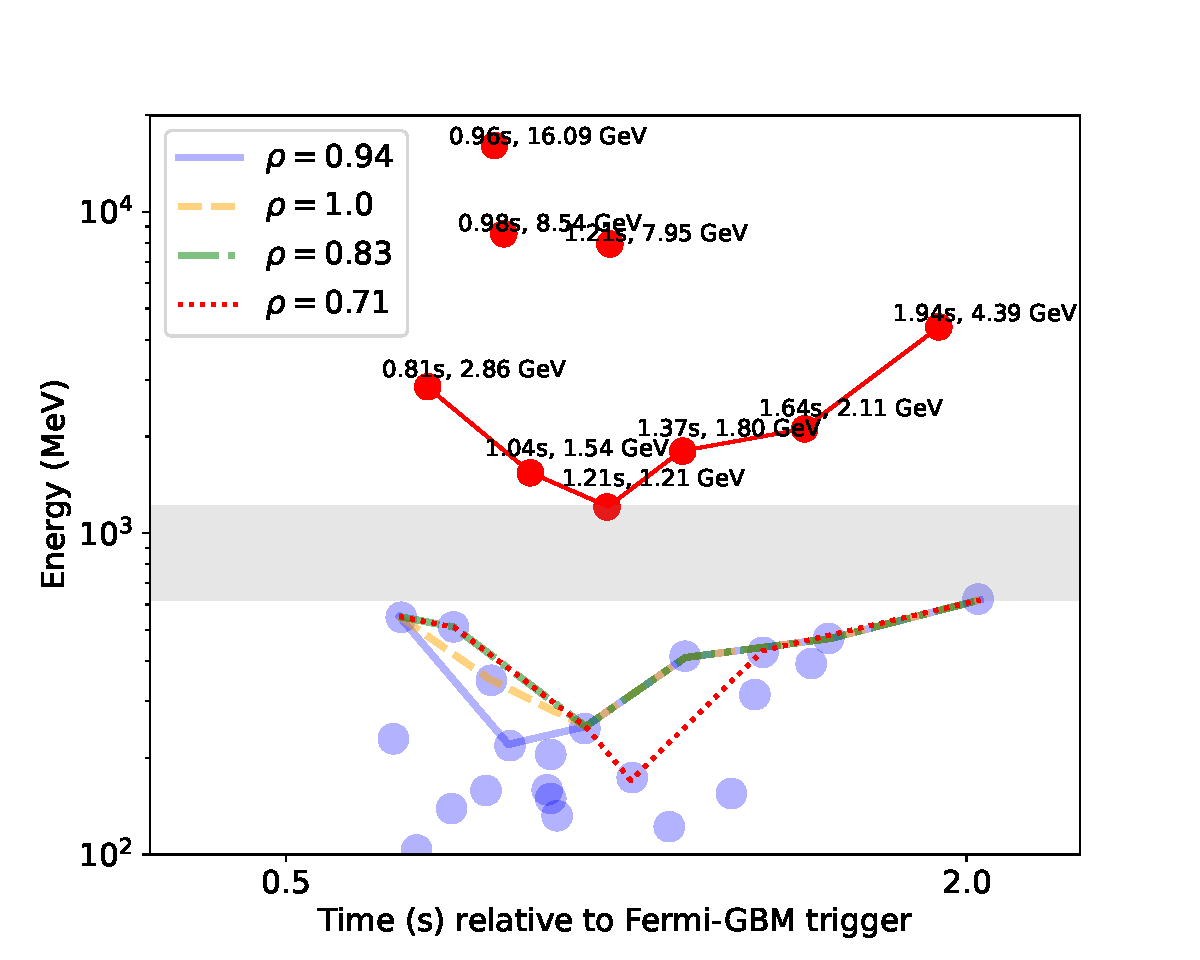
\includegraphics[width=.49\textwidth]{EvsT_LAT0p5_2p2_2.pdf}\\
\caption{The Spearman rank correlation coefficients of temporal evolution between $\gamma^{\rm envelope}_{\rm GeV}$ and $\gamma^{\rm envelope}_{\rm sub-GeV}$ (denoted by different line styles and colors) extracted with different bin-edge division ratios. The gray shadow between 0.62 and 1.21 GeV shows the intersection of all gaps between sub-GeV and GeV photons.\label{fig:correlation}}
 \end{center}
\end{figure} 


\section{The possible correlation between $\gamma^{\rm envelope}_{\rm sub-GeV}$ and $\gamma^{\rm envelope}_{\rm GeV}$}\label{sec: correlation}

The Spearman rank correlation coefficient ($\rho$)~\citep{spearman}\footnote{The \DIFdelbegin \DIFdel{spearman }\DIFdelend \DIFaddbegin \DIFadd{Spearman }\DIFaddend rank correlation coefficient $\rho$ is defined as $\rho = \frac{\mathrm{cov}(r(x),r(y))}{\sigma_x \sigma_y} $ where $r(a)$ represents the rank of element $a$. For non-duplicated datasets, $\rho$ can be interpreted as $\rho = 1 - \frac{6 \Sigma d^2_i}{n(n^2-1)} $ where $d_i = r(x) - r(y)$.} is used to quantify the monotonic relationship of the temporal evolution between the energy of $\gamma^{\rm envelope}_{\rm GeV}$ (denotes the lower envelope of GeV photons) and that of $\gamma^{\rm envelope}_{\rm sub-GeV}$ (denotes the upper energy envelope of sub-GeV photons). $\gamma^{\rm envelope}_{\rm GeV}$ is naturally formed by the GeV photons as shown in FIG.~\ref{fig:correlation} in red circles connected by a red line.
In order to ensure a one-to-one correspondence between $\gamma^{\rm envelope}_{\rm sub-GeV}$ and $\gamma^{\rm envelope}_{\rm GeV}$, the maximum sub-GeV energy value in each time bin was extracted as $\gamma^{\rm envelope}_{\rm sub-GeV}$; the data binning in the range of $T_0+[0.70, 2.05]$ s is performed as follows: 1) the edges of the bin are determined to be the n-equal division points in time of each adjacent GeV point in $\gamma^{\rm envelope}_{\rm GeV}$; 2) to reduce the impact of artificial selection, the bin-edge division ratio (rate) is tested from 0.01 to 0.99 with an increment of 0.01 (for example, a rate equal to 0.2 means left five-division point). 

From all binning results with different bin-edge division ratios, four different energy envelopes of sub-GeV photons were extracted, as shown in FIG.\DIFaddbegin \DIFadd{~}\DIFaddend \ref{fig:correlation}. $\rho$ is determined to be $> 0.7$ conservatively from \DIFaddbegin \DIFadd{the }\DIFaddend results of all sets of bin edges, which implies a strong correlation between $\gamma^{\rm envelope}_{\rm sub-GeV}$ and $\gamma^{\rm envelope}_{\rm GeV}$\footnote{The grading standards and the corresponding correlation degrees are available online:~\href{https://www.statstutor.ac.uk/resources/uploaded/spearmans.pdf}{Spearman's correlation}. }.
\section{Spectral \DIFdelbegin \DIFdel{Modelings }\DIFdelend \DIFaddbegin \DIFadd{modelings }\DIFaddend with different models and the analysis \DIFdelbegin \DIFdel{for }\DIFdelend \DIFaddbegin \DIFadd{of }\DIFaddend the prompt emission}\label{sec:spectra2}
% FIG.~\ref{fig:spectra2} shows the time-integrated spectral modeling result with mBB + BAND without the gap bin, which is marked in gray in (a). Plots (c)-(e) are Modeling results with BAND, BB+BAND, and mBB+PL respectively.
FIG.~\ref{fig:spectra2} shows the time-integrated spectral modeling results with mBB + \DIFdelbegin \DIFdel{BAND, mBB }\DIFdelend \DIFaddbegin \DIFadd{PL, BAND }\DIFaddend + PL and \DIFdelbegin \DIFdel{BAND }\DIFdelend \DIFaddbegin \DIFadd{mBB }\DIFaddend + \DIFdelbegin \DIFdel{PL}\DIFdelend \DIFaddbegin \DIFadd{BAND}\DIFaddend .
The parameters of the three best models are listed below (BIC and $\chi^2$ \DIFdelbegin \DIFdel{to the degree }\DIFdelend \DIFaddbegin \DIFadd{over the degrees }\DIFaddend of freedom are shown in the figures)\DIFdelbegin \DIFdel{,
}\DIFdelend \DIFaddbegin \DIFadd{:
}\DIFaddend \begin{itemize}
    \item BAND+PL: for the BAND component, $\alpha=-0.06^{+0.14}_{-0.11}$, $\beta=-2.80^{+0.26}_{-0.35}$, $E_{\rm p}=256.1^{+13.4}_{-16.1}$ keV, $F_{\rm BAND}=10.7^{+0.7}_{-0.7}\times10^{-6}$ erg cm$^{-2}$ s$^{-1}$; for the PL component: index $p=-1.80^{+0.18}_{-0.09}$, $F_{\rm PL}=20.2^{+3.7}_{-4.2}\times10^{-6}$ erg cm$^{-2}$ s$^{-1}$; 
    \item mBB+PL: for the mBB component, $m=-0.29^{+0.37}_{-0.37}$, $kT_{\rm min}=19.1^{+3.0}_{-3.5}$ keV, $kT_{\rm max}=146.0^{+25.2}_{-17.3}$ keV, $F_{\rm mBB}=8.5^{+0.4}_{-0.3}\times10^{-6}$ erg cm$^{-2}$ s$^{-1}$; for the PL component: $p=-1.81^{+0.06}_{-0.03}$, $F_{\rm PL}=22.4^{+5.6}_{-5.6}\times10^{-6}$ erg cm$^{-2}$ s$^{-1}$; 
    \item mBB+BAND: for the mBB component, $m=-0.37^{+0.55}_{-0.60}$, $kT_{\rm min}=18.8^{+3.7}_{-5.3}$ keV, $kT_{\rm max}=145.1^{+20.0}_{-14.1}$ keV, $F_{\rm mBB}=7.7^{+0.4}_{-0.4}\times10^{-6}$ erg cm$^{-2}$ s$^{-1}$; 
    for the BAND component: $\alpha=-1.68^{+0.04}_{-0.02}$, $\beta=-1.90^{+0.16}_{-0.07}$, \DIFdelbegin \DIFdel{log10($E_{\rm p})=3.89^{+0.17}_{-0.14}$ keV}\DIFdelend \DIFaddbegin \DIFadd{$\log_{10}(E_{\rm p}/{\rm keV})=3.89^{+0.17}_{-0.14}$}\DIFaddend , $F_{\rm BAND}=23.3^{+1.7}_{-1.8}\times10^{-6}$ erg cm$^{-2}$ s$^{-1}$.
\end{itemize}
From the residual distribution \DIFdelbegin \DIFdel{of }\DIFdelend \DIFaddbegin \DIFadd{from }\DIFaddend 40 keV to 300 keV, there exists a systematic bias in the modeling with \DIFaddbegin \DIFadd{the }\DIFaddend BAND + PL functions. The change \DIFdelbegin \DIFdel{on }\DIFdelend \DIFaddbegin \DIFadd{in }\DIFaddend BIC is $\Delta$BIC = 8.1, which shows a strong preference for mBB + PL. Therefore, the mBB function is better than the BAND function for describing the MeV peak component from the modeling results. In addition, the low-energy photon index for the peaking component is about \DIFdelbegin \DIFdel{-0.1}\DIFdelend \DIFaddbegin \DIFadd{$-0.1$}\DIFaddend , although it cannot be decisive evidence for the quasi-thermal emission. The $\Delta$BIC of mBB+BAND \DIFaddbegin \DIFadd{relative }\DIFaddend to mBB+PL is 1.8\DIFdelbegin \DIFdel{, and }\DIFdelend \DIFaddbegin \DIFadd{; although }\DIFaddend BAND is not an \DIFdelbegin \DIFdel{unconventional }\DIFdelend \DIFaddbegin \DIFadd{unreasonable }\DIFaddend model for the component of the broad energy band\DIFdelbegin \DIFdel{; thus}\DIFdelend , the mBB + BAND model is not better than mBB + PL.

It is evident that there exist two different components in the prompt emission. There are two candidate processes to interpret the observation:


1) There exist seed photons in the outflow, and some of them become the component of a broad energy band from keV to GeV via inverse Compton (IC) scattering by relativistic electrons. However, not all \DIFaddbegin \DIFadd{of them }\DIFaddend are emitted, especially \DIFdelbegin \DIFdel{for }\DIFdelend those with lower energies, which correspond to a larger scattering cross section with electrons; moreover, as \DIFdelbegin \DIFdel{electrons are cooled}\DIFdelend \DIFaddbegin \DIFadd{the electrons cool}\DIFaddend , the cross section of electron-photon scattering becomes larger and even increases to the Thomson cross section ($\sigma_{\rm T}>\sigma_{\rm KN}$). They will be thermalized below the photosphere and emitted when the radius reaches $R_{\rm ph}$; $R_{\rm ph}$ satisfies ($r_0$ is the initial radius for jet launching, and ranges from $10^7$ cm to $10^9$ cm)~\citep{2018pgrb.book.....Z}
\begin{eqnarray}
    R_{\rm ph}&\simeq&(\frac{L_{\rm K}\sigma_{\rm e\gamma}}{8\pi m_pc^3\Gamma})^{1/3} r_0^{2/3}\nonumber\\
    &=&4.9\times10^{11}L_{\rm K,55} ^{1/3} (\frac{\sigma_{\rm e\gamma}}{\sigma_{\rm T}})^{1/3}\Gamma_{2.7}^{-1/3}r^{2/3}_{0,8}\ \rm cm %\nonumber
 \end{eqnarray}
 for the unsaturated acceleration regime; for the saturated acceleration regime,
 \begin{eqnarray}
 R_{\rm ph}&\simeq&\frac{L_{\rm K}\sigma_{\rm e\gamma}}{8\pi m_pc^3\Gamma^3}\nonumber\\
    &=& 4.7\times10^{13}L_{\rm K, 55} (\frac{\sigma_{\rm e\gamma}}{\sigma_{\rm T}}) \Gamma_{2.7}^{-3}\ \rm cm.
\end{eqnarray}
The observed time delay \DIFdelbegin \DIFdel{$\simeq(1+z)R_{\rm ph}/2c\Gamma^2$ for $R_{\rm ph}\lesssim10^{11-13}$ cm }\DIFdelend \DIFaddbegin \DIFadd{of this component }\DIFaddend relative to the \DIFdelbegin \DIFdel{keV to GeV component}\DIFdelend \DIFaddbegin \DIFadd{keV--GeV component, $\simeq(1+z)R_{\rm ph}/(2c\Gamma^2)$, }\DIFaddend is less than a few milliseconds \DIFaddbegin \DIFadd{for $R_{\rm ph}\lesssim10^{11}-10^{13}$ cm}\DIFaddend . This means that \DIFaddbegin \DIFadd{the }\DIFaddend two components arrive almost simultaneously, which is consistent with the observation. \DIFaddbegin \DIFadd{(We have also used the cross-correlation function to obtain the time lag between the emission below 20 keV, where the contamination from the quasi-thermal component is less than $7\%$, and that in 50--100 keV; the lag is determined to be around 0. Although the prompt emission is a superposition of the two components, this implies that there is no very large time delay between them.)
}\DIFaddend 

2) The synchrotron self-Compton (SSC) process in the internal shocks could also account for the two components in the prompt phase. The peaking MeV component comes from synchrotron emission of the accelerated electrons, while some of them behave as seed photons for the IC scattering. However, \DIFdelbegin \DIFdel{peak }\DIFdelend \DIFaddbegin \DIFadd{the peaking }\DIFaddend MeV emission should not be quasi-thermal since $\tau_{\rm KN}<1$, which is not consistent with the modeling results that the mBB function is better than the BAND function in describing \DIFaddbegin \DIFadd{the }\DIFaddend peak MeV emission. \DIFaddbegin \DIFadd{Secondly, given $L_{\gamma,\rm peak}\simeq4\times10^{53}$ erg s$^{-1}$ in $T_0+[0.7, 2.05]$ s, similar fractions of the electron and magnetic-field energies, and $E_{\rm p}\sim250$ keV, the typical Lorentz factor of the emitting electrons is estimated following \mbox{%DIFAUXCMD
\cite{2011ApJ...726...90Z}}\hskip0pt%DIFAUXCMD
; $\gamma_{e,\rm p}\gtrsim10^{3.5}$ requires the peaking component to be emitted at a large radius ($R\sim10^{14}$ cm) so that $\tau_{\rm KN}(E_{\rm obs}\sim250~{\rm keV})<1$ is satisfied, whereas at such a large radius the optical depth for the photodissociation of the deuteron would be much less than 1.
}\DIFaddend 

Thus, we think that the first explanation is more consistent with the observations. \DIFaddbegin \DIFadd{In addition, because most of the energy in the prompt phase is contributed by the keV--GeV component ($L_{\gamma,\rm keV-GeV}=1.0\times10^{54}$ erg s$^{-1}$, about 2.6 times that of the peaking component, $L_{\gamma,\rm peak}\simeq3.7\times10^{53}$ erg s$^{-1}$), and $L_{\rm K}$ is estimated from this component, the emission mechanism of the MeV peaking component does not affect the calculation and conclusion much.
}\DIFaddend 



\begin{figure*}
\begin{center}
 \centering
%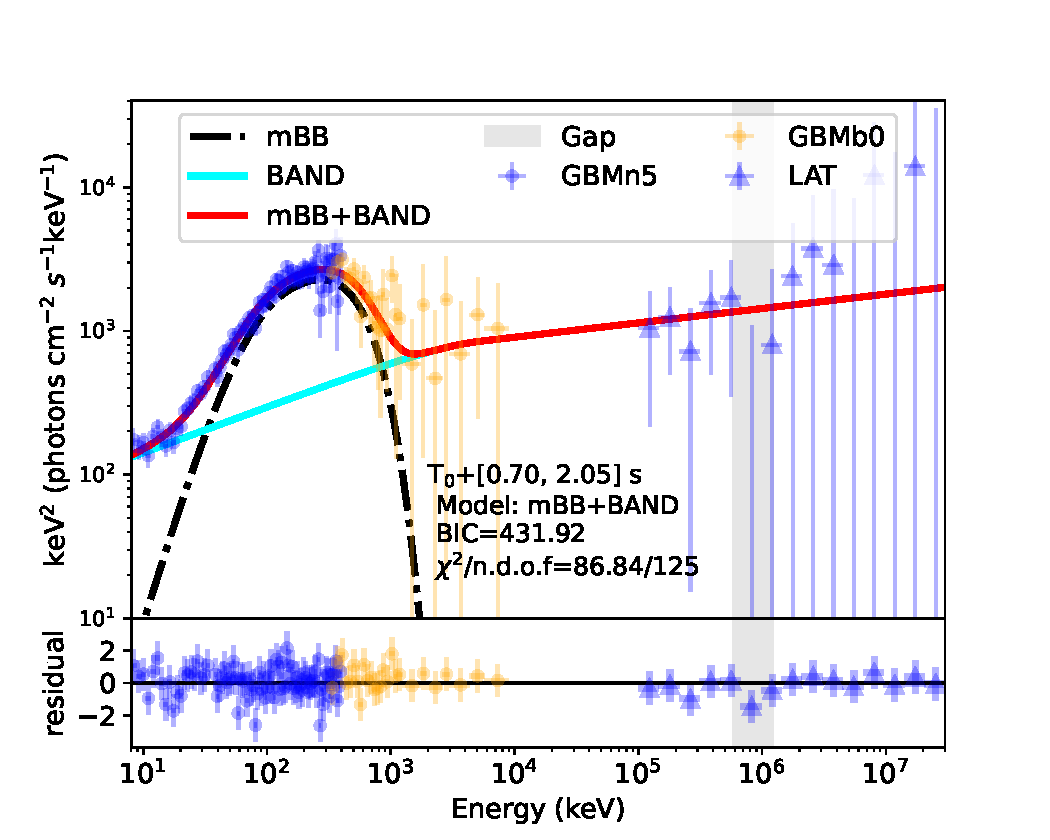
\includegraphics[width=.47\textwidth]{Fv_mBBBAND0_GRB210704A_withgapbin.pdf}\put(-110,130){(a) }

%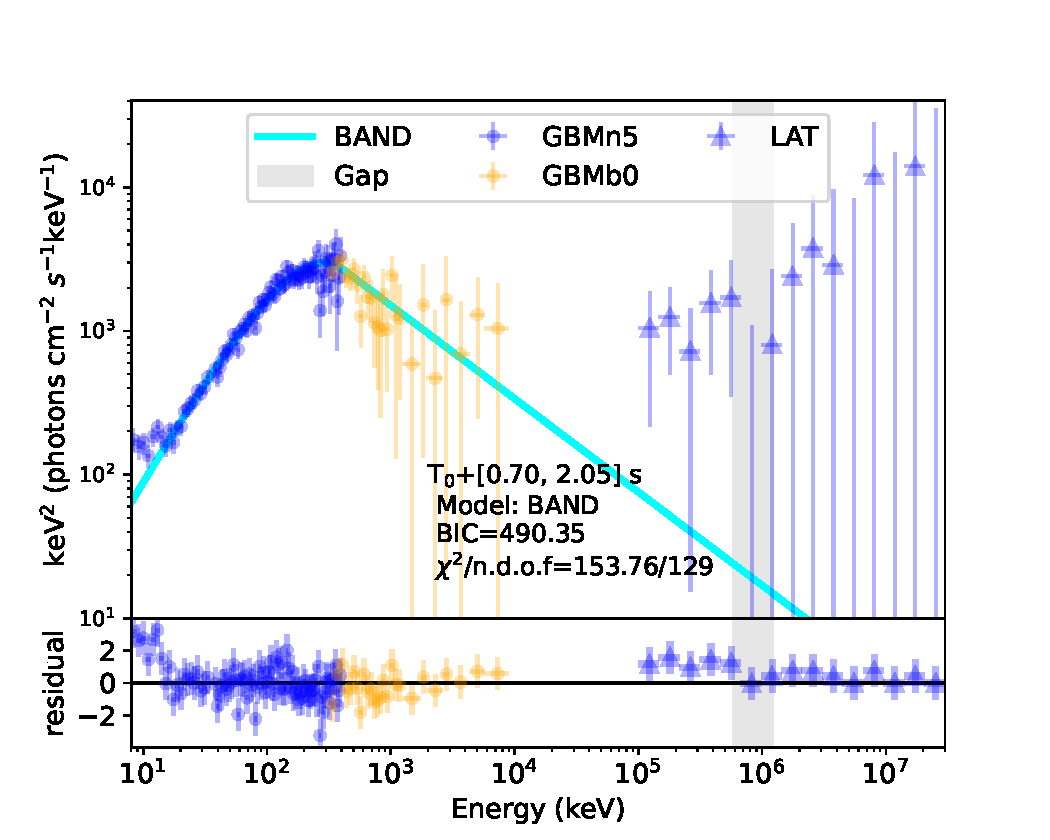
\includegraphics[width=.47\textwidth]{Fv_BAND0_GRB210704A.pdf}\put(-110,130){(b) }\\
%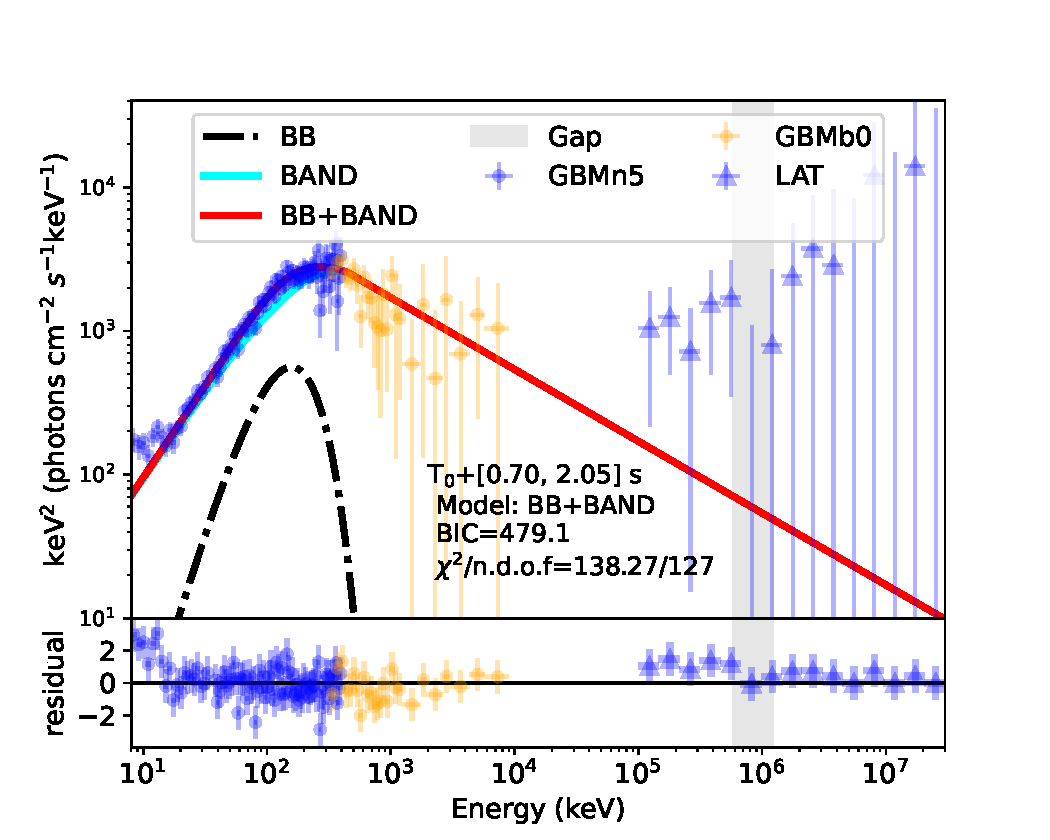
\includegraphics[width=.47\textwidth]{Fv_BBBAND0_GRB210704A.pdf}\put(-110,130){(c) }
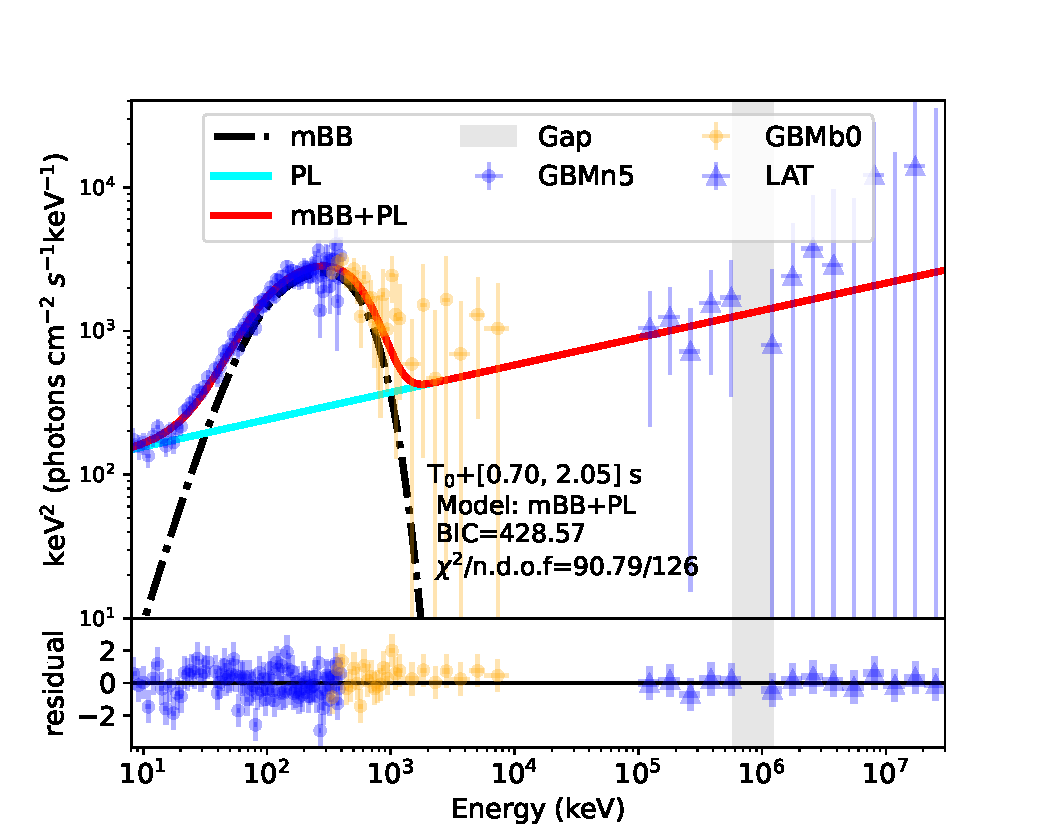
\includegraphics[width=.47\textwidth]{Fv_mBBPL0_GRB210704A.pdf}\put(-110,130){(a) }
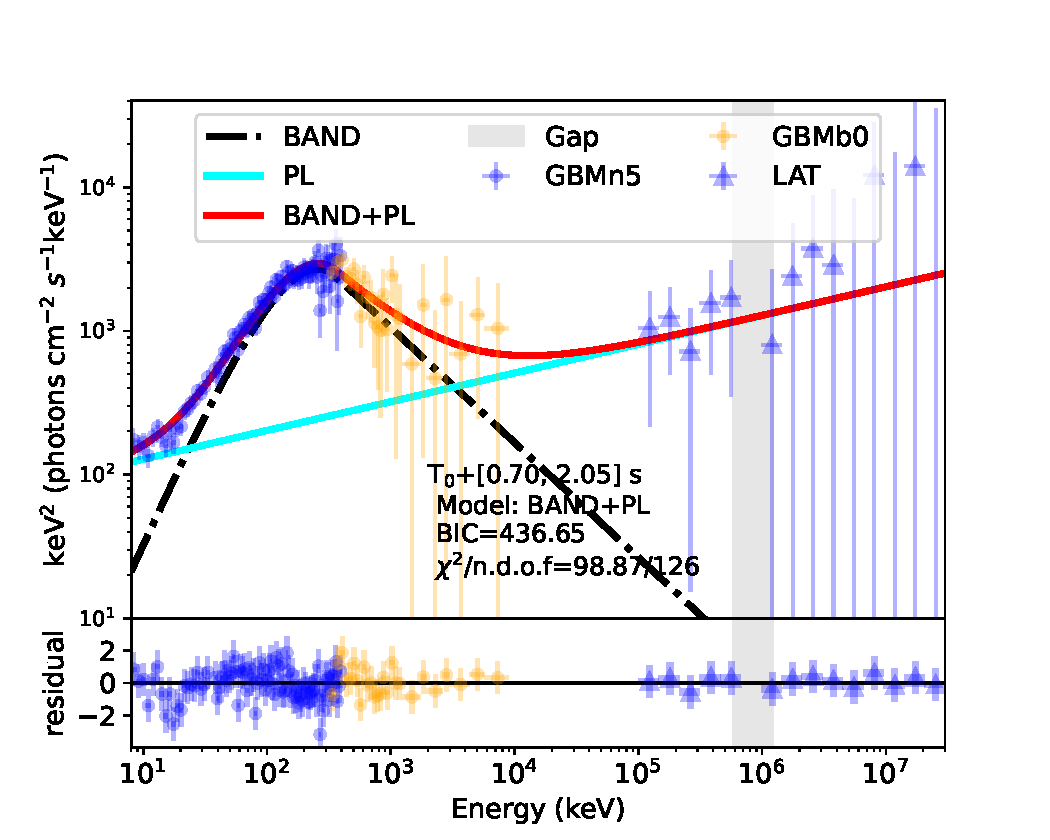
\includegraphics[width=.47\textwidth]{Fv_BANDPL0_GRB210704A.pdf}\put(-110,130){(b) }\\
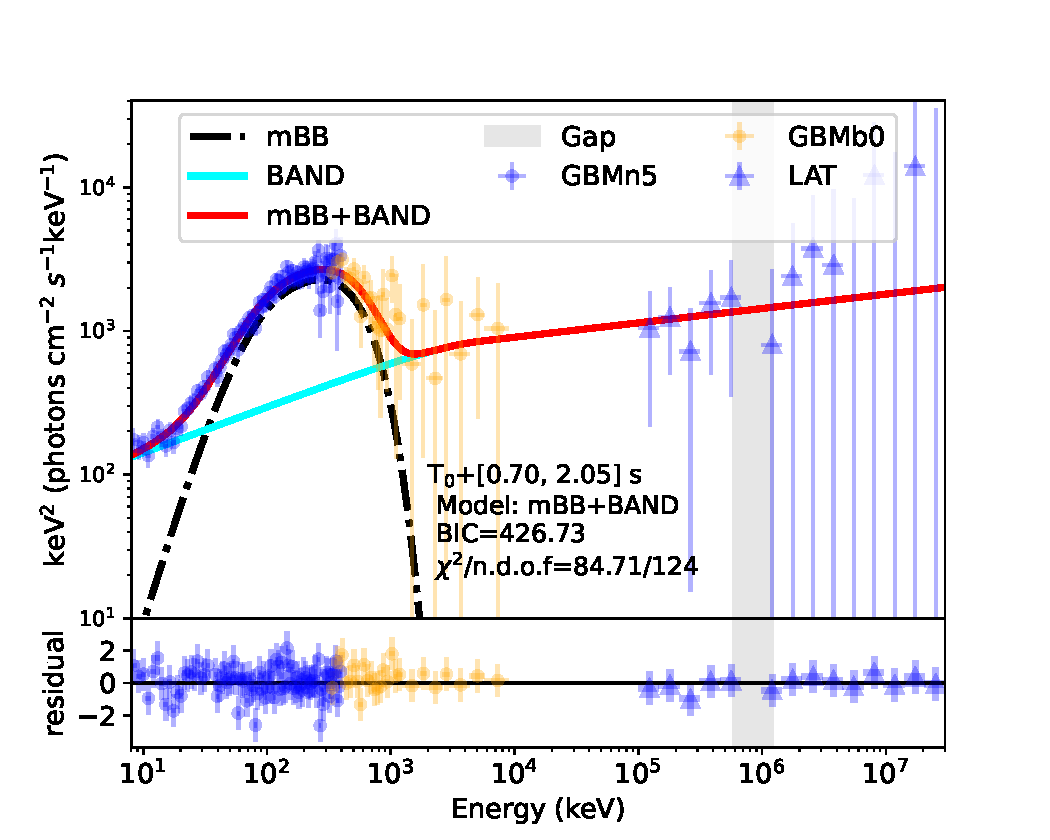
\includegraphics[width=.47\textwidth]{Fv_mBBBAND0_GRB210704A.pdf}\put(-110,130){(c) }
\caption{\label{fig:spectra2} (Color online) Modeling results with \DIFaddbeginFL \DIFaddFL{(a) }\DIFaddendFL mBB+\DIFdelbeginFL \DIFdelFL{BAND}\DIFdelendFL \DIFaddbeginFL \DIFaddFL{PL}\DIFaddendFL , \DIFdelbeginFL \DIFdelFL{mBB}\DIFdelendFL \DIFaddbeginFL \DIFaddFL{(b) BAND}\DIFaddendFL +PL and \DIFdelbeginFL \DIFdelFL{BAND }\DIFdelendFL \DIFaddbeginFL \DIFaddFL{(c) mBB}\DIFaddendFL +\DIFdelbeginFL \DIFdelFL{PL, }\DIFdelendFL \DIFaddbeginFL \DIFaddFL{BAND; the }\DIFaddendFL bins inside the gap (gray) are excluded from the fits.}
    \end{center}
\end{figure*}

\section{The estimates of $\Gamma$} \label{sec: estiGamma}

\subsection{Estimate of the Range of $\Gamma$ with quasi-thermal emission}
The approach for the estimate of $\Gamma$ is sketched in broad terms in the typical fireball model of GRBs~\citep[e.g.][]{1986ApJ...308L..47G,1986ApJ...308L..43P} as follows: the thermal component originates from the photosphere of an
expanding plasma jet; the observed thermal flux (integrated over
all frequencies) is given by integrating the intensity over the
emitting \DIFaddbegin \DIFadd{surface}\DIFaddend ~\citep{2007ApJ...664L...1P},
\begin{equation}\label{eq:Fobs_BB}
  F^{\rm obs}_{\rm BB} = \frac{2\pi}{d_L^2} \int^{\mu_{\rm max}}_{\mu_{\rm min}} d\mu \mu
r_{ph}^2 \D^4 (\sigma_{\rm SB} T'^4_{\rm ph} / \pi).  
\end{equation}
 Here, $T'_{\rm ph}$ is the comoving
temperature at the photospheric radius, $\sigma_{\rm SB}$ is Stefan's
constant and $\D = \D(\theta)$ is the Doppler factor, $\D =
[\Gamma(1-\beta \mu)]^{-1}$. The angle $\theta$ is the angle
between the direction of the outflow velocity vector ($\beta$) and
the line of sight, $\mu \equiv \cos(\theta)$, and $\Gamma = (1-
\beta^2)^{-1/2}$ is the outflow Lorentz factor.  
The observed radiation is dominated by photons
emitted close to the line of sight ($\theta_{\rm min}=0$), the upper integration
boundary in the equation for the thermal flux is $\mu_{\rm max}=\cos \theta_{\rm min}=1$, thus one has~\citep{2007ApJ...664L...1P, 2015ApJ...801..103G}:
\begin{eqnarray}
T_{\rm obs}& = & C_1\Gamma_{\rm ph} T'_{\rm ph} /(1+z),\\
F^{\rm obs}_{\rm BB} & = & \mathcal{R}^2\sigma_{\rm SB} T_{\rm obs}^4,
\end{eqnarray}
where
\begin{eqnarray}
\mathcal{R}=C_2~\frac{(1+z)^2}{d_L}\frac{r_{\rm ph}}{\Gamma_{\rm ph}};
\end{eqnarray}
 $C_1 \simeq 1.48$ and $C_2 \simeq 1.06$ are factors derived from the detailed numerical integration of the angle- and distance-dependent photosphere emission. 


Taking into account different regimes of acceleration of the outflow, for example, in the case of saturation regime (i.e. $r_{\rm ph}$ is greater than $r_{\rm s}$, and $r_s$ is the saturation radius), $r_{\rm ph}=L\sigma_{\rm T}/8\pi \Gamma^3 m_p c^3$ (here $L=4\pi d^2_{\rm L }Y F^{\rm obs}$, $Y\geq 1$ is the ratio between the total energy and the energy emitted in $\gamma$-rays, $F^{\rm obs}$ is the sum of thermal and non-thermal component; $\Gamma=\eta$, where $\eta$ is the dimensionless \DIFdelbegin \DIFdel{entropy}\DIFdelend \DIFaddbegin \DIFadd{enthalpy}\DIFaddend ), one has
\begin{equation}
    \Gamma = \left[(1.06) { (1+z)^2 d_L} {Y F^{\rm obs} \sigma_T \over 2 m_p
    c^3 \R} \right]^{1/4}.
\label{eq:eta}
\end{equation}


More realistically, the observed spectra are broader than the Planck spectrum, because of geometrical broadening~\citep[e.g.][]{2008ApJ...682..463P}. This means that the observed spectrum is a superposition of a series of blackbodies of different temperatures arising from different angles to the line of sight; therefore, a multi-blackbody (mBB) function could be used to describe the quasi-thermal spectrum, and the
temperatures of the individual Planck function are related
by a power law. In addition, the other component of the outflow (i.e., Poynting flux) also affects the estimate of $\Gamma$. Therefore, this approach is extended based on basic physical models (the so-called `top-down' approach; see the details in \DIFdelbegin \DIFdel{\mbox{%DIFAUXCMD
\citep{2015ApJ...801..103G} }\hskip0pt%DIFAUXCMD
and \mbox{%DIFAUXCMD
\citep{2024ApJ...961..137S}}\hskip0pt%DIFAUXCMD
}\DIFdelend \DIFaddbegin \DIFadd{\mbox{%DIFAUXCMD
\citealt{2015ApJ...801..103G} }\hskip0pt%DIFAUXCMD
and \mbox{%DIFAUXCMD
\citealt{2024ApJ...961..137S}}\hskip0pt%DIFAUXCMD
}\DIFaddend ). %In this case of mBB function, $kT_{\rm max}$ and $F_{\rm max}= F_{\rm mBB}/(1-(\frac{kT_{\rm min}}{kT_{\rm max}})^{q})$ could be taken as a good probe for the properties of the outflow; $kT_{\rm max}$, $kT_{\rm min}$ and  $q=m+1$ could be extracted from the modeling with data. 
Note that in \DIFdelbegin \DIFdel{an }\DIFdelend \DIFaddbegin \DIFadd{the }\DIFaddend unsaturated regime, $\Gamma$ \DIFdelbegin \DIFdel{, }\DIFdelend \DIFaddbegin \DIFadd{and }\DIFaddend $r_{\rm ph}$ are related to the initial radius $r_0$\DIFdelbegin \DIFdel{, }\DIFdelend \DIFaddbegin \DIFadd{; }\DIFaddend physically $r_0=10^7 - 10^9$ cm, \DIFdelbegin \DIFdel{therefore }\DIFdelend \DIFaddbegin \DIFadd{from which }\DIFaddend the range of \DIFaddbegin \DIFadd{the }\DIFaddend $\Gamma$ value is estimated.
\DIFdelbegin %DIFDELCMD < \iffalse
%DIFDELCMD < %%%
\DIFdelend \subsection{Estimate of \DIFaddbegin \DIFadd{the }\DIFaddend lower limit of $\Gamma$ with the photon with the highest energy}
\DIFdelbegin %DIFDELCMD < 

%DIFDELCMD <  %%%
\DIFdelend \DIFaddbegin \label{sec:gammalowlimit}
 \DIFaddend The optical depth for pair production of a high-energy photon (with observed energy of $E_{\rm GeV, obs}$) in the jet with the Lorentz factor $\Gamma$ at a radius $R_{\gamma\gamma}$ is defined as
\DIFdelbegin \begin{displaymath}\DIFdel{%DIFDELCMD < \label{eq:taugg}%%%
\tau_{\gamma\gamma}\simeq \sigma_{\gamma\gamma} n^{'}_{\gamma, >E_{\pm, \rm obs}}R_{\gamma\gamma} /\Gamma   
}\end{displaymath}%DIFAUXCMD
\DIFdelend \DIFaddbegin \begin{equation}\DIFadd{\label{eq:taugg}
\tau_{\gamma\gamma}\simeq \sigma_{\gamma\gamma} n^{'}_{\gamma, >E_{\pm, \rm obs}}R_{\gamma\gamma} /\Gamma,
}\end{equation}\DIFaddend 
 where $\sigma_{\gamma\gamma}$ ($\sim10^{-25}$ cm$^{2}$) is the cross section of $\gamma\gamma\rightarrow e^{+}+e^{-}$, and $n^{'}_{\gamma, >E_{\pm,\rm obs}}$ is the number density of the target photons in the comoving frame; the observed energy $E_{\pm, \rm obs}$ of these target photons should satisfy the following criterion (note that an on-axis observation is assumed),
\begin{equation}\label{eq:Eobs}
 E_{\pm, \rm obs}>\left(\frac{2\Gamma m_ec^2}{1+z}\right)^2\frac{1}{E_{\rm GeV, obs}}.
\end{equation}
The distribution of photons in the MeV-energy band could be described by $f(E_{\rm obs})$ (with a normalization factor $K$ and a unit of keV$^{-1}$ cm\DIFdelbegin \DIFdel{$^{-1}$ }\DIFdelend \DIFaddbegin \DIFadd{$^{-2}$ }\DIFaddend s$^{-1}$). We have %The luminosity ($L(E_{\rm obs})$) is given by
\begin{eqnarray}\label{eq:Eobs2}
     4\pi d^2_{\rm L}\int_{E_{\pm,\rm obs}}^\infty Kf(E)dE =4\pi R_{\gamma\gamma}^2 c n_{\gamma, >E_{\pm,\rm obs}}(1+z),
\end{eqnarray}
where in the frame of the observer $n_{\gamma, >E_{\pm,\rm obs}}=2\Gamma n^{'}_{\gamma, >E_{\pm,\rm obs}}$\DIFdelbegin \DIFdel{. 
%DIF < and $R_{\gamma\gamma}$ could be given by %Note that  $\Gamma=260$ is large enough for $\gamma_{16.1 \rm GeV}$ to be emitted with a small time delay ($\Delta t$) relative to MeV photons, as described by
}\DIFdelend \DIFaddbegin \DIFadd{, and $R_{\gamma\gamma}$ could be given by
}\begin{equation}\DIFadd{\label{eq:Rgg}
   R_{\gamma\gamma}\simeq R_{\rm ph} +2c\Gamma^2\Delta t/(1+z),
}\end{equation}
\DIFadd{where $\Delta t$ is the arrival time delay of high-energy photons relative to the MeV emission.
With Eqs.~(\ref{eq:taugg})-(\ref{eq:Rgg}), in the one-zone assumption (i.e., if the GeV photons were produced in the same region as the MeV photons), the requirement $\tau_{\gamma\gamma}<1$ for the emission of the photon with the highest energy (16.09 GeV) around the peak flux would provide a lower limit of $\Gamma\gtrsim500$ at $R_{\gamma\gamma}\sim10^{11}$ cm. Note that in this method the estimated $\Gamma$ is approximately proportional to $(1+z)$, so the comoving energies are almost unaffected by the choice of the redshift. This one-zone assumption is relaxed in the two-zone configuration discussed in the next subsection.
}\DIFaddend 

\DIFdelbegin \begin{displaymath}\DIFdel{%DIFDELCMD < \label{eq:Rgg}%%%
   R_{\gamma\gamma}\simeq R_{\rm ph} +(1+z)2c\Gamma^2\Delta t,
}\end{displaymath}%DIFAUXCMD
\DIFdelend \DIFaddbegin \subsection{\DIFadd{Two-zone constraint on the Lorentz factor of the GeV-emitting region}}
\label{sec:twozone}
%DIF > %% Numerical results in this subsection are produced by twozone_crossing_gaozou.py, adapted from the published code of Gao & Zou (2023), github.com/qilunuo9/two-zone_model; the transcription reproduces their Table 1 for GRB 221009A (297.7/161.7/139.4/113.0 vs the published 297.92/162.93/139.31/113.06 at t_T = 5/10/15/20 s).
\DIFadd{The one-zone limit derived above assumes that the GeV photons are produced in the same region as the MeV photons. In our model they originate from different internal shocks: the MeV emission comes from an inner region (radius $R_{\rm M}$, Lorentz factor $\Gamma_{\rm M}$), while the GeV photons come from a more external internal shock (radius $R_{\rm G}$, Lorentz factor $\Gamma_{\rm G}$). Since the outer region is still an internal shock, its radius is set by the millisecond variability timescale, $R_{\rm G}=2\Gamma_{\rm G}^{2}c\,\delta t/(1+z)\sim10^{12}$ cm, rather than by the much larger external-shock radius considered for GRB 221009A in \mbox{%DIFAUXCMD
\cite{2023ApJ...956L..38G}}\hskip0pt%DIFAUXCMD
; it is thus of the same order as the radius at which $\tau_{\gamma D}$ and $\tau_{\rm KN}$ are evaluated in the main text. In this configuration a GeV photon does not encounter the bright MeV radiation field at its production site: it overtakes the MeV photon shell at $R>R_{\rm G}$, where the MeV photons move almost radially, and the collision angle decreases along the trajectory as $R\sin\theta=R_{\rm G}\sin\theta_{\rm G}$, which strongly reduces the pair-production opacity compared with the one-zone case~\mbox{%DIFAUXCMD
\citep{2011ApJ...726L...2Z,2023ApJ...956L..38G}}\hskip0pt%DIFAUXCMD
.
}

\DIFadd{Following \mbox{%DIFAUXCMD
\cite{2011ApJ...726L...2Z} }\hskip0pt%DIFAUXCMD
with the corrections of \mbox{%DIFAUXCMD
\cite{2023ApJ...956L..38G} }\hskip0pt%DIFAUXCMD
(the TeV zone there corresponds to our GeV zone here), the simplified analytic expression for the minimum Lorentz factor of the GeV region reads
}\begin{equation}\DIFadd{\label{eq:GGmin}
\Gamma_{\rm G,min}\approx\left[\frac{(1+z)^{2\alpha-3}L_{\rm M}\,\epsilon_{\rm G}^{\alpha-1}\,\epsilon_{\rm P}^{\alpha}\,\sigma_{\rm T}}{12\times4^{\alpha}\,\pi\,m_{\rm e}c^{4}\,t_{\rm G}\,\epsilon_{\rm P}^{*2}\,\alpha}\right]^{\frac{1}{2\alpha+2}},
}\end{equation}
\DIFadd{where $\epsilon\equiv E/(m_{\rm e}c^{2})$, $t_{\rm G}\simeq\delta t\simeq1$ ms is the emission timescale of the GeV region, $E_{\rm P}^{*}$ is the effective peak energy }[\DIFadd{Eq.~(8) of \mbox{%DIFAUXCMD
\citealt{2023ApJ...956L..38G}}\hskip0pt%DIFAUXCMD
}]\DIFadd{, and $\alpha$ is the photon index of the MeV target spectrum at the pair-production threshold. For the photon with the highest energy (16.09 GeV), the threshold, $\approx1$ MeV in the observer frame, lies above $E_{\rm p}=256$ keV, so the relevant index is the high-energy Band index of the MeV component, $\alpha=\beta_{\rm M}=2.80$ (the MeV peaking component can be fitted by a Band function as well as by the mBB model); Eq.~(\ref{eq:GGmin}) then gives $\Gamma_{\rm G,min}\approx1.0\times10^{3}$. In this regime the threshold falls on the steep high-energy wing of the Band spectrum, where the single-power-law and cross-section approximations behind Eq.~(\ref{eq:GGmin}) overestimate the opacity, so the analytic value should be regarded as an upper estimate. The full formulas }[\DIFadd{Eqs.~(12)-(13) of \mbox{%DIFAUXCMD
\citealt{2023ApJ...956L..38G}}\hskip0pt%DIFAUXCMD
}]\DIFadd{, integrated numerically with the exact pair-production cross section and the Doppler-weighted average over the emission angle, give the reliable limit
}\begin{equation}
\DIFadd{\Gamma_{\rm G,min}\simeq4.3\times10^{2},\qquad R_{\rm G}\simeq3.4\times10^{12}\ {\rm cm}.
}\end{equation}\DIFaddend 
\DIFdelbegin %DIFDELCMD < \fi
%DIFDELCMD < %%%
%DIF < where $\Delta t$ is the arrival time delay of high-energy photons relative to MeV emission. 
\DIFdelend 

\DIFdelbegin \subsection{\DIFdel{Estimation based on statistical correlation}}
%DIFAUXCMD
\addtocounter{subsection}{-1}%DIFAUXCMD
\DIFdel{There are empirical correltions between $\Gamma$ and $E_{\rm iso}$ and $L_{\rm iso}$:
}\DIFdelend \DIFaddbegin \DIFadd{With $\Gamma_{\rm G}\simeq(3-4.3)\times10^{2}$, the observed gap (}[\DIFadd{0.62, 1.21}] \DIFadd{GeV) translates to a comoving energy of $\approx2.4-6.7$ MeV, which brackets the photodissociation resonance of deuterium, and $R_{\rm G}\simeq(1-3)\times10^{12}$ cm is of the same order as the radius at which $\tau_{\gamma D}\gtrsim1$ is obtained in the main text; the escape of the highest-energy photon and the resonant deuterium absorption are therefore consistent within the same region. The photons of $1.21-4.39$ GeV that constitute the upper boundary of the gap have higher pair-production thresholds, where the MeV target photons are much rarer, and thus yield much weaker constraints. The corresponding two-zone constraint on the inner MeV region is much weaker still, because the collision angle for the photons emitted along the line of sight is limited by the small angular size of the inner source \mbox{%DIFAUXCMD
\citep{2011ApJ...726L...2Z}}\hskip0pt%DIFAUXCMD
; the Lorentz factor of the photospheric outflow is instead characterized by the quasi-thermal estimate above (500-900).
%DIF > %% TODO(team): (1) the adopted typical value Gamma = 10^2.5 in the main text lies slightly below the 16.09-GeV requirement Gamma_G >~ 4.3e2; at Gamma_G ~= 434 (R_G ~= 3.4e12 cm) tau_gD from the main-text formula needs the per-pulse enhancement of L_K (or a larger Y_D) to remain >~ 1 -- reconcile the numbers, or attribute the single 16 GeV photon to the upper end of the window. (2) The co-spatial (self) absorption of the 16 GeV photon on the outer zone's own PL photons is not relieved by the two-zone geometry; it is resolved by the outer zone's own ~MeV luminosity being very weak, to be substantiated from the spectral fits (the bright ~MeV emission belongs to the inner quasi-thermal zone) -- per Y.-C. Zou, to be added separately.
}

%DIF > \subsection{Estimation based on statistical correlation}
%DIF > There are empirical correlations between $\Gamma$ and $E_{\rm iso}$ and $L_{\rm iso}$: %%% TODO: this subsection was left unfinished; either complete it (e.g., with the $\Gamma_0-E_{\gamma,\rm iso}$ and $\Gamma_0-L_{\gamma,\rm iso}$ relations of Liang et al. 2010, ApJ 725, 2209 and L\"u et al. 2012, ApJ 751, 49, which are currently not in LIV.bib) or leave it removed.
\DIFaddend 


\subsection{The estimate of $\Gamma$ in GRB 210704A}
The \DIFdelbegin \DIFdel{ranges }\DIFdelend \DIFaddbegin \DIFadd{range }\DIFaddend of $\Gamma$ is estimated in different regimes using the `top-down' approach. Regime II ($r_{\rm ra}<r_{\rm ph}<r_{\rm c}$, where $r_{\rm ra}$ is the rapid acceleration radius, and $r_{\rm c}$ is the coasting radius) is allowed. For $T_0+[0.70, 2.05]$ s and assuming $Y=10$, $\Gamma$ ranges from 500 to 900. Note that from Eq\DIFaddbegin \DIFadd{.}\DIFaddend ~(\ref{eq:eta}), $\Gamma\propto Y^{1/4}$\DIFdelbegin \DIFdel{, }\DIFdelend \DIFaddbegin \DIFadd{; }\DIFaddend the value of $Y$ does not affect the estimate of $\Gamma$ much, e.g., the factor of $Y^{1/4}$ \DIFdelbegin \DIFdel{of }\DIFdelend \DIFaddbegin \DIFadd{for }\DIFaddend $Y=10$ is 1.5 times that \DIFdelbegin \DIFdel{of }\DIFdelend \DIFaddbegin \DIFadd{for }\DIFaddend $Y=2$. %DIF < In fact, $\Gamma$ is determined from modeling with a specific model (e.g., a top-hat afterglow model; see the details in ~\citep{2026MNRAS.548ag555P}) to be about $1000 \pm 600$, which means the result of approach is consistent with the model-dependent estimation of afterglow.
\DIFaddbegin \DIFadd{In fact, $\Gamma$ determined from the modeling with a specific model (e.g., a top-hat afterglow model; see the details in \mbox{%DIFAUXCMD
\citealt{2026MNRAS.548ag555P}}\hskip0pt%DIFAUXCMD
) is about $1000 \pm 600$, which means that the result of this approach is consistent with the model-dependent estimation from the afterglow.
}\DIFaddend 

%With Eqs~(\ref{eq:taugg})-(\ref{eq:Eobs2}), $\tau_{\gamma\gamma}<1$ of 1.21 GeV photon emitted requires $\Gamma\gtrsim1000$ for $R=10^{13}$ cm. Thus, the above estimate of $500\lesssim\Gamma\lesssim 900$ is large enough for the almost simultaneous emission of high-energy photons.

%In addition, $\Gamma$ of merged shell in the internal shock model should be between the maximum and minimum values.
%Thus, we take $500< \Gamma <900$ to be a reasonable range for the shell.




%\clearpage
\bibliography{LIV}
\bibliographystyle{apsrev4-2}

\end{document}